\exercisegroup

\begin{enumerate}
\def\labelenumi{\arabic{enumi})}
\item
  Let \(\mathrm{F}, \mathrm{G}\) be two vector spaces in duality, such that \(\sigma(\mathrm{F}, \mathrm{G})\) is Hausdorff. Show that if \(\mathcal{T}\) is a Hausdorff topology compatible with the vector space structure of \(\mathrm{F}\) and coarser than \(\sigma(\mathrm{F}, \mathrm{G})\) (but not necessarily locally convex a priori), then \(\mathcal{T} = \sigma(\mathrm{F}, \mathrm{G}_1)\) , where \(\mathrm{G}_1\) is a vector subspace of G, dense in the topology \(\sigma(\mathrm{G},\mathrm{F})\) . (Consider on F the locally convex topology \(T_{1}\) in which a fundamental system of neighbourhoods of 0 is formed by the closed, convex, balanced sets in T which are neighbourhoods of 0 for \(\sigma(\mathrm{F},\mathrm{G})\) .) Deduce that if \(T_{0}\) is a Hausdorff locally convex topology on a vector space E, that is minimal in the set of Hausdorff locally convex topologies on E (II, p.~85, exerc. 13) it is also minimal in the set of topologies (locally convex or not) that are Hausdorff and compatible with the vector space structure of E.
\item
  In \(\mathbf{R}^n\) , let \((\mathrm{C}_i)_{1\leqslant i\leqslant m}\) be a family of \(m\geqslant n + 1\) convex cones with vertex 0; show that if, for any \(n + 1\) of these cones there exists a hyperplane \(\mathbf{H}\) through 0 and such that the cones lie on the same side of \(\mathbf{H}\) , then there exists a hyperplane \(\mathrm{H}_0\) such that all the cones \(\mathrm{C}_i(1\leqslant i\leqslant m)\) lie on the same side of \(\mathrm{H}_0\) (cf.~II, p.~68, exerc. 21, a)).
\item
  In \(\mathbf{R}^n\) let \((\mathrm{D}_i)_{1\leqslant i\leqslant m}\) be a family of \(m\geqslant 2n\) closed half-spaces determined by hyperplanes passing through 0. Show that if, for any \(2n\) of these half spaces, there exists a point \(\neq 0\) in their intersection, then there exists a point \(\neq 0\) in the intersection of all the \(\mathrm{D}_i(1\leqslant i\leqslant m)\) (cf.~II, p.~66, exerc. 10).
\item
  Let S, T be two finite sets in \(R^{n}\) , without common points, such that their union contains at least \(2n + 2\) points. Then there exists a hyperplane separating S from T if, and only if, for every finite set \(F \subset S \cup T\) of \(2n + 2\) points, there exists a hyperplane separating \(F \cap S\) from \(F \cap T\) (use exerc. 3 and the method of II, p.~78, exerc. 15).
\item
  Let E be the vector space of quadratic forms on \(R^{n}\) , which is identified with the vector subspace of symmetric square matrices in the space \(\mathbf{M}_{n}(\mathbf{R})\) of square matrices of order n on R. We endow \(\mathbf{M}_{n}(\mathbf{R})\) with the scalar product \(\operatorname{Tr}(^{t}\mathbf{X},\mathbf{Y})\) , which enables us to identify it with its dual and similarly for E.
\end{enumerate}

\begin{enumerate}
\def\labelenumi{\alph{enumi})}
\item
  Let \(\mathbf{P} \subset \mathbf{E}\) be the set of quadratic forms for which the matrix has all elements \(\geqslant 0\) , and let \(\mathbf{S} \subset \mathbf{E}\) be the set of positive quadratic forms in \(\mathbf{R}^n\) . Show that we have \(\mathbf{P} = \mathbf{P}^\circ\) and \(\mathbf{S} = \mathbf{S}^\circ\) .
\item
  Let B be the set of quadratic forms on \(\mathbf{R}^n\) that can be written in the form \(\sum_{j=1}^{m} x_j'^2\) for same \(m\) , where \(x_{j}^{\prime}\) is a linear form that takes values \(\geqslant 0\) for all \(x = (x_{i})_{1\leqslant i\leqslant n}\) of coordinates \(x_{i}\) all \(\geqslant 0\) ; let \(C\) be the set of quadratic forms that are \(\geqslant 0\) for all the vectors \(x = (x_{i})\) with coordinates \(x_{i}\) all \(\geqslant 0\) . Show that \(B = C^{\circ}\) and \(C = B^{\circ}\) (prove that \(B\) is closed, showing that every element of \(B\) can be written in the form \(\sum_{j=1}^{m} x_{j}^{\prime 2}\) , with \(x_{j}^{\prime}\) positive for all \(x\) with coordinates \(\geqslant 0\) , and \(m \leqslant 2^{n}\) ).
\end{enumerate}

\begin{enumerate}
\def\labelenumi{\arabic{enumi})}
\setcounter{enumi}{5}
\tightlist
\item
  Let F, G be two vector spaces in separating duality, and A a weakly compact convex set in F. Let C be a convex cone with vertex 0, that is weakly closed in G. Suppose that, for all \(y \in \mathbf{C}\) , there exists \(x \in \mathbf{A}\) such that \(\langle x, y \rangle \geqslant 0\) . Show that there exists \(x_0 \in \mathbf{A}\) such that \(\langle x_0, y \rangle \geqslant 0\) for all \(y \in \mathbf{C}\) (apply prop. 4 of II, p.~38, to A and \(\mathbf{C}^\circ\) ).
\end{enumerate}

¶ 7) a) Let F, G be two vector spaces in separating duality and C a weakly closed convex cone in F. Let M be a finite dimensional vector subspace of G. Show that, either there exists \(y_0 \in \mathbf{C}\) such that \(y_0 \in \mathbf{M}^\circ\) and \(y_0 \neq 0\) , or there exists \(z_0 \in \mathbf{M}\) such that \(z_0 \in \mathbf{C}^\circ\) and \(z_0 \neq 0\) (argue by induction on the dimension of M). If C does not contain any line and if the two preceding properties are simultaneously satisfied, show that \(z_0\) cannot be an internal point of \(\mathbf{C}^\circ\) . b) Let the two matrices \((a_{ij}), (b_{ij})\) with real entries in \(n\) rows and \(m\) columns, be such that \(a_{ij} > 0\) for every pair \((i,j)\) . Show that there is a unique value of \(\lambda \in \mathbf{R}\) such that there are two vectors \(x = (x_j) \in \mathbf{R}^m\) , \(y = (y_i) \in \mathbf{R}^n\) satisfying the relations \(x \neq 0, y \neq 0, x_j \geqslant 0, y_i \geqslant 0\) for all \(i,j\) and finally such that

\[
\lambda \sum_ {j = 1} ^ {m} a _ {i j} x _ {j} \geqslant \sum_ {j = 1} ^ {m} b _ {i j} x _ {j} \quad \text { for } \quad 1 \leqslant i \leqslant n\tag{1}
\]

\[
\lambda \sum_ {i = 1} ^ {n} a _ {i j} y _ {i} \leqslant \sum_ {i = 1} ^ {n} b _ {i j} y _ {i} \quad \text { for } \quad 1 \leqslant j \leqslant m\tag{2}.
\]

(Putting \(c_{ij} = \lambda a_{ij} - b_{ij}\) for \(1 \leqslant i \leqslant n\) , \(1 \leqslant j \leqslant m\) , and \(c_{n + i,j} = \delta_{ij}\) (Kronecker's index) for \(1 \leqslant i \leqslant m\) show that the problem reduces to finding a vector \(x \in \mathbf{R}^m\) and a vector \(z = (z_i) \in \mathbf{R}^{n + m}\) which are non null and satisfy the relations

\[
\sum_ {j = 1} ^ {m} c _ {i j} x _ {j} \geqslant 0 \quad \text { for } \quad 1 \leqslant i \leqslant n + m\tag{3}
\]

\[
\sum_ {i = 1} ^ {n + m} c _ {i j} z _ {i} = 0 \quad \text { for } \quad 1 \leqslant j \leqslant m\tag{4}
\]

and \(z_{i} \geqslant 0\) for \(1 \leqslant i \leqslant n + m\) . Remark that, if (3) has a solution for one value \(\lambda_0\) of \(\lambda\) , then it also has a solution for \(\lambda \geqslant \lambda_0\) , and that if (4) has a solution for \(\lambda_0\) , then it also has a solution for \(\lambda \leqslant \lambda_0\) . Finally use \(a)\) .

\begin{enumerate}
\def\labelenumi{\arabic{enumi})}
\setcounter{enumi}{7}
\tightlist
\item
  Let \(\mathbf{T}\) be a compact space and \(\mathbf{L}\) a vector subspace of \(\mathcal{C}(\mathbf{T};\mathbf{R})\) , that is of finite dimension \(r\) ; give to \(\mathbf{L}\) the norm induced by that of \(\mathcal{C}(\mathbf{T};\mathbf{R})\) and to its dual \(\mathbf{L}^*\) the norm \(\| x'\| = \sup_{\| x\| \leqslant 1} \langle x, x' \rangle\) , so that if \(\mathbf{B}\) is the ball \(\| x\| \leqslant 1\) in \(\mathbf{L}\) , then \(\mathbf{B}^\circ\) is the ball \(\| x'\| \leqslant 1\) in \(\mathbf{L}^*\) .
\end{enumerate}

\begin{enumerate}
\def\labelenumi{\alph{enumi})}
\tightlist
\item
  For all \(t \in \mathbf{T}\) , write \(e_t'\) for the linear form \(x \mapsto x(t)\) on \(\mathbf{L}\) . Show that \(\mathbf{B}^\circ\) is the convex envelope of the set of the \(\pm e_t'\) , where \(t\) varies in \(\mathbf{T}\) (obtain a contradiction using prop. 4 of II, p.~38).
\end{enumerate}

Deduce that every linear form \(x' \in \mathbf{L}^*\) such that \(\| x' \| = 1\) we can write \(x' = \sum_{i=1}^{r} \lambda_i e_{t_i}'\) , where

the \(t_i\) are \(r\) points of \(\mathbf{T}\) and the \(\lambda_i\) are real numbers such that \(\sum_{i=1}^{r} |\lambda_i| = 1\) (cf.~II, p.~66, exerc. 9, a)).

\begin{enumerate}
\def\labelenumi{\alph{enumi})}
\setcounter{enumi}{1}
\tightlist
\item
  For every \(y \in \mathcal{C}(\mathbf{T}; \mathbf{R})\) , there exists a unique \(x \in \mathbf{L}\) such that \(\| y - x \| = d(y, \mathbf{L})\) , if and only if for every non null \(z \in \mathbf{L}\) , there exist at most \(r - 1\) distinct points \(t_i \in \mathbf{T}\) such that \(z(t_i) = 0\) (Haar's th.). (To show that this condition is sufficient, observe first that it is equivalent to saying that for \(r\) distinct points \(t_i \in \mathbf{T}\) ( \(1 \leqslant i \leqslant r\) ) the \(e_{t_i}'\) are linearly independent in \(\mathbf{L}^*\) . Now argue by assuming the conclusion is false and obtaining a contradiction. If there exist two distinct points \(x', x''\) of \(\mathbf{L}\) such that \(\| y - x' \| = \| y - x'' \| = d(y, \mathbf{L})\) then there exists \(x_0 \in \mathbf{L}\) and \(z \in \mathbf{L}\) such that, for all sufficiently small real \(\lambda\) , we have \(\| y - (x_0 + \lambda z) \| = d(y, \mathbf{L})\) . Apply the last part of \(a\) ) to the subspace \(\mathbf{L} \oplus \mathbf{R}y\) of \(\mathcal{C}(\mathbf{T}; \mathbf{R})\) and to a suitable linear form on this space which vanishes in \(\mathbf{L}\) . To see that the condition is necessary, note that if it is not true, then there exist \(r\) distinct points \(t_i \in \mathbf{T}\) ( \(1 \leqslant i \leqslant r\) ) such that the \(e_{t_i}'\) are linearly dependent and there exists a function \(z \in \mathbf{L}\) that is not null and vanishes at the points \(t_i\) . If \(\alpha_i (1 \leqslant i \leqslant r)\) are numbers not all zero such that \(\sum_{i=1}^{r} \alpha_i e_{t_i}' = 0\) , consider a function \(w \in \mathcal{C}(\mathbf{T}; \mathbf{R})\) such that \(\| w \| = 1\) , \(w(t_i) = \text{sgn}(\alpha_i)\) for \(1 \leqslant i \leqslant r\) , and the function \(y = w(1 - |\beta z|)\) with \(|\beta|\) sufficiently small and \(\neq 0\) .)
\item
  Suppose that \(T\) is a compact interval in \(R\) and that \(L\) satisfies the condition of Haar's th.; let \((t_i)_{1 \leqslant i \leqslant r+1}\) be a strictly increasing sequence of \(r + 1\) points of \(T\) ; then there exist \(r + 1\) real non zero numbers \(\lambda_i\) such that \(\sum_{i=1}^{r+1} \lambda_i e_{t_i}' = 0\) . Show that then \(\text{sgn}(\lambda_i) \text{sgn}(\lambda_{i+1}) = -1\) for \(1 \leqslant i \leqslant r\) . (Consider separately the case \(r = 1\) and the case \(r > 1\) . In the second case, suppose on the contrary, that for some index \(i \leqslant r - 1\) , the number \(\lambda_i\) is of the same sign as \(\lambda_{i-1}\) or as \(\lambda_{i+1}\) and that \(\lambda_{i-1}\) and \(\lambda_{i+1}\) are of opposite signs. If, for example, \(\lambda_i > 0\) , take \(\alpha_{i-1} > 0\) , \(\alpha_{i+1} > 0\) such that \(\alpha_{i-1} \lambda_{i-1} + \alpha_{i+1} \lambda_{i+1} = 0\) , then \(z \in L\) such that \(z(t_{i-1}) = \alpha_{i-1}\) , \(z(t_{i+1}) = \alpha_{i+1}\) and \(z(t_j) = 0\) for \(j\) distinct from \(i - 1, i\) and \(i + 1\) . Deduce that \(z(t_i) < 0\) and show that this contradicts the given hypotheses.)
\end{enumerate}

\(d)\) With the same hypotheses and notations as those of \(c\) ), suppose that there exists \(y \in \mathcal{C}(\mathrm{T}; \mathbf{R})\) and \(z \in \mathrm{L}\) such that \(y(t_i) - z(t_i) = (-1)^i \alpha_i\) with \(\alpha_i > 0\) for \(1 \leqslant i \leqslant r + 1\) . Show that we then have \(d(y, \mathrm{L}) \geqslant \inf \alpha_i\) . (Use \(a\) ) applied to \(\mathrm{L} \oplus \mathbf{R}y\) , and \(c\) .)

\begin{enumerate}
\def\labelenumi{\alph{enumi})}
\setcounter{enumi}{4}
\tightlist
\item
  With the hypotheses of \(c\) let \(y \in \mathcal{C}(\mathbf{T};\mathbf{R})\) , and \(z\) be the unique point of \(\mathbf{L}\) such that \(\| y - z \| = d(y,\mathbf{L})\) . Show that there exists a strictly increasing sequence \((t_i)_{1\leqslant i\leqslant r + 1}\) in \(\mathbf{T}\) such that
\end{enumerate}

\[
y (t _ {i}) - z (t _ {i}) = (- 1) ^ {i} \varepsilon \| y - z \|
\]

with \(\varepsilon = \pm 1\) . Conversely if \(z\) has this property, then \(z\) is the unique point of \(\mathbf{L}\) such that \(\| y - z \| = d(y, \mathbf{L})\) . (Use \(c\) ) and \(d\) ). Consider the case when \(\mathbf{T}\) is an interval of \(\mathbf{R}\) and when \(\mathbf{L}\) is the set of the restrictions to \(\mathbf{T}\) of polynomials of degree \(< r\) ( \(Tchebycheffs\) th.).

\begin{enumerate}
\def\labelenumi{\arabic{enumi})}
\setcounter{enumi}{8}
\tightlist
\item
  Let \(\mathbf{F}\) and \(\mathbf{G}\) be two vector spaces in separating duality and \(\mathbf{A}\) be a convex subset of \(\mathbf{F}\) which contains 0. For every \(y \in \mathbf{G}\) , write
\end{enumerate}

\[
\mathrm{H} _ {\mathbf {A}} (y) = \sup _ {x \in \mathbf {A}} (- \langle x, y \rangle),
\]

so that \(0 \leqslant \mathrm{H}_{\mathbf{A}}(y) \leqslant +\infty\) ; we call \(\mathrm{H}_{\mathbf{A}}\) the support function of \(\mathbf{A}\) .

\begin{enumerate}
\def\labelenumi{\alph{enumi})}
\item
  Show that \(\mathbf{H}_{\mathrm{A}}\) is the gauge of \(\mathbf{A}^{\circ}\) (II, p.~20).
\item
  If A is weakly compact, then, for all \(y \in \mathbf{G}\) , the hyperplane with the equation \(\langle x, y \rangle = \mathrm{H}_{\mathbf{A}}(y)\) is a support hyperplane of A.
\item
  \(\mathbf{H}_{\mathrm{A}}\) is finite and continuous for the topology \(\sigma (\mathbf{G},\mathbf{F})\) if, and only if, A is finite-dimensional and bounded (in the finite dimensional vector subspace that it generates).
\end{enumerate}

\(d\) ) Let \(\mathbf{A}_i(1\leqslant i\leqslant p)\) be convex sets in F which contain 0 and \(\lambda_{i}\) be real numbers \(\geqslant 0(1\leqslant i\leqslant p)\) ; show that the support function of the convex set \(\mathbf{A} = \sum_{i}\lambda_{i}\mathbf{A}_{i}\) is \(\mathrm{H}_{\mathrm{A}} = \sum_{i}\lambda_{i}\mathrm{H}_{\mathrm{A}_{i}}\) . If \(y\in \mathbf{G}\) is

such that the intersection \(C_{i}\) , of \(A_{i}\) with the hyperplane \(\langle x, y \rangle = H_{A}(y)\) , is non-empty for \(1 \leqslant i \leqslant p\) , show that the intersection of A and the hyperplane with equation \(\langle x, y \rangle = H_{A}(y)\) is the set \(\sum \lambda_{i}C_{i}\) .

\begin{enumerate}
\def\labelenumi{\alph{enumi})}
\setcounter{enumi}{4}
\item
  Suppose that \(\mathbf{A}\) is locally compact and does not contain any line. Then the set which is the union of \(\{0\}\) and the set of \(y \neq 0\) such that \(\mathrm{H}_{\mathrm{A}}(y) = +\infty\) , \(\mathrm{H}_{\mathrm{A}}(-y) \neq +\infty\) is the polar cone of the asymptotic cone \(\mathrm{C}_{\mathrm{A}}\) (consider the case when \(\mathbf{A}\) is the convex envelope of \(\{0\}\) and of one half-line).
\item
  Suppose that F is finite dimensional. Show that, A is parabolic (II, p.~67, exerc. 17) if and only if \(H_{A}\) is a continuous mapping of G in \(\overline{R}\) (if there exists a line parallel to a half-line of \(C_{A}\) , which does not meet A, note that there exists a hyperplane separating this half-line from A).
\end{enumerate}

\begin{enumerate}
\def\labelenumi{\arabic{enumi})}
\setcounter{enumi}{9}
\tightlist
\item
  To each compact convex set A in \(E = R^{n}\) containing 0, we make correspond its support function \(H_{A}\) by the duality between E and \(E^{*} : H_{A}\) belonging to the space \(\mathcal{C}(E^{*}; \mathbf{R})\) of continuous real valued functions in \(E^{*}\) . We ascribe to the space \(\mathcal{C}(E^{*}; \mathbf{R})\) the uniform structure of compact convergence and, to the set \(\Re_{0}^{\prime}(E)\) of the compact convex sets in E containing 0, the uniform structure defined in the exerc. 39 of II, p.~71. Show that \(A \mapsto H_{A}\) is an isomorphism of \(\Re_{0}^{\prime}(E)\) on a uniform subspace of \(\mathcal{C}(E^{*}; \mathbf{R})\) .
\end{enumerate}

Deduce that the mapping \(\mathbf{A} \mapsto \mathbf{A}^{\circ}\) of the set \(\Re_0(\mathbf{E})\) of compact convex sets in \(\mathbf{E}\) which contain 0 as an interior point, on the set \(\Re_0(\mathbf{E}^*)\) , is an isomorphism for the uniform structures of these two spaces (cf.~II, p.~71, exerc. 39).

\begin{enumerate}
\def\labelenumi{\arabic{enumi})}
\setcounter{enumi}{10}
\tightlist
\item
  Let \(\mathrm{F}, \mathrm{G}\) be two vector spaces in separating duality. An ultrafilter \(\mathfrak{U}\) on \(\mathrm{F}\) converges weakly to a point \(x_0\) if, and only if, \(x_0\) belongs to the intersection of all the weakly closed convex sets which belong to \(\mathfrak{U}\) (note that if \(x_0\) is a point of this intersection that is not a cluster point of \(\mathfrak{U}\) , then there exists a closed half-space belonging to \(\mathfrak{U}\) and not containing \(x_0\) ).
\end{enumerate}

Deduce from this result that, for a sequence of points \((x_{n})\) of F to be weakly convergent to a point a, it is necessary and sufficient that a belongs to all the weakly closed convex envelopes of the sets formed by an infinity of the terms of the sequence (use prop. 7 of GT, I, § 6.4).

\begin{enumerate}
\def\labelenumi{\arabic{enumi})}
\setcounter{enumi}{11}
\tightlist
\item
  \begin{enumerate}
  \def\labelenumii{\alph{enumii})}
  \tightlist
  \item
    Let E be a vector space and \((\mathrm{E}_{\alpha})_{\alpha\in\mathrm{A}}\) be an increasing directed family of subspaces of E, whose union is E; each \(E_{\alpha}\) is supposed to carry a locally convex topology \(T_{\alpha}\) such that for \(\alpha\leqslant\beta\) the canonical injection \(E_{\alpha}\to E_{\beta}\) is continuous. Let T be the topology on E, which is the inductive limit of the \(T_{\alpha}\) (II, p.~29, Example II); show that the dual \(E'\) of E (for T) with the topology \(\sigma(\mathrm{E}',\mathrm{E})\) can be canonically identified with the projective limit of the duals \(E'_{\alpha}\) , with topology \(\sigma(\mathrm{E}'_{\alpha},\mathrm{E}_{\alpha})\) .
  \end{enumerate}
\end{enumerate}

\begin{enumerate}
\def\labelenumi{\alph{enumi})}
\setcounter{enumi}{1}
\tightlist
\item
  Let \((\mathbf{X}_{\alpha},\phi_{\alpha \beta})\) be a projective system of non-empty sets corresponding to a directed set of indices A, such that \(\phi_{\alpha \beta}\) are surjective and that \(\varprojlim \mathbf{X}_{\alpha} = \emptyset\) \((\mathbf{S},\mathbf{III},\S 7,\text{exerc. }4)\) . Put \(\mathbf{F}_{\alpha} = \mathbf{R}^{(\mathbf{X}_{\alpha})}\) and denote by \(f_{\alpha \beta}:\mathrm{F}_{\beta}\to \mathrm{F}_{\alpha}\) for \(\alpha \leqslant \beta\) the linear mapping deduced canonically from \(\phi_{\alpha \beta}\) (A, II, § 1.11, cor. 1). If, we give to each \(\mathbf{F}_{\alpha}\) the topology which is the direct sum topology of its factors, the dual \(\mathrm{E}_{\alpha} = \mathrm{F}_{\alpha}'\) of \(\mathrm{F}_{\alpha}\) , with the weak topology \(\sigma(\mathrm{E}_{\alpha}, \mathrm{F}_{\alpha})\) , can be identified with the product space \(\mathbf{R}^{\mathbf{X}_{\alpha}}\) , and \({}^{t}f_{\alpha\beta}\) is an isomorphism of \(\mathrm{E}_{\alpha}\) on a closed subspace of \(\mathrm{E}_{\beta}\) , having a topological complement in \(\mathrm{E}_{\beta}\) . Show that on \(\mathrm{E} = \varinjlim \mathrm{E}_{\alpha}\) (for the \({}^{t}f_{\alpha\beta}\) ) the topology which is the inductive limit of those of \(\mathrm{E}_{\alpha}\) is the coarsest topology (therefore non-Hausdorff) (using \(a\) ) and noting that \(\varprojlim \mathrm{F}_{\alpha} = \{0\}\) ).
\end{enumerate}

\begin{enumerate}
\def\labelenumi{\arabic{enumi})}
\setcounter{enumi}{12}
\tightlist
\item
  Let E be a vector space. We say that a Hausdorff locally convex topology T on E is minimal (and that E, with T, is a space of minimal type) if there exists no Hausdorff locally convex topology on E, that is strictly coarser than T (cf.~II, p.~81, exerc. 1).
\end{enumerate}

\begin{enumerate}
\def\labelenumi{\alph{enumi})}
\item
  Let \(\mathcal{T}\) be a minimal topology on E, and let \(E'\) be the dual of E (when E has the topology \(\mathcal{T}\) ); show that \(\mathcal{T} = \sigma(E, E')\) and \(E = E'^*\) (note that there cannot be an everywhere dense hyperplane in \(E'\) for the topology \(\sigma(E', E)\) using the cor. 3 of II, p.~43). Deduce that spaces of minimal type are products of lines.
\item
  Show that in a Hausdorff locally convex space F, every subspace E of minimal type has a topological complement, and in particular is closed (use a) and the Hahn-Banach th. for extending the identity mapping of E in itself to a mapping of F in E).
\item
  Let \(u\) be a continuous linear mapping of a space \(\mathbf{E}\) of minimal type in a Hausdorff locally convex space \(\mathbf{F}\) . Show that \(u(\mathbf{E})\) is closed in \(\mathbf{F}\) and that \(u\) is a strict morphism of \(\mathbf{E}\) in \(\mathbf{F}\) (use \(b\) ) and the definition of a space of minimal type).
\item
  Let F be a Hausdorff locally convex space and M be a closed vector subspace of F. Show that, if there exists a complement N of M in F that is a subspace of minimal type, then N is a topological complement of M in F (use c)).
\item
  Let M be a subspace of minimal type in a Hausdorff locally convex space F; show that, for every closed vector subspace N of F the sum \(M + N\) is closed in F (consider the quotient space F/N and use c)). If further N is of minimal type, then \(M + N\) is of minimal type.
\end{enumerate}

\begin{enumerate}
\def\labelenumi{\arabic{enumi})}
\setcounter{enumi}{13}
\tightlist
\item
  Let \(\mathbf{E}\) be a Hausdorff locally convex space and \(\mathbf{F}\) a locally convex space of minimal type (exerc. 13).
\end{enumerate}

\begin{enumerate}
\def\labelenumi{\alph{enumi})}
\item
  Show that if \(\mathbf{M}\) is a closed vector subspace of the product space \(\mathrm{E} \times \mathrm{F}\) , its projection on \(\mathrm{E}\) is closed in \(\mathrm{E}\) (use exerc. 13, e)).
\item
  Let \(u\) be a linear mapping of \(\mathbf{E}\) in \(\mathbf{F}\) . Show that if the graph of \(u\) is closed in \(\mathbf{E} \times \mathbf{F}\) , then \(u\) is continuous (use \(a\) ).
\item
  Suppose that, in E, every closed vector subspace has a topological complement (cf.~V, p.~13). Show that, in \(E \times F\) , every closed vector subspace M has a topological complement. (If \(N_{1}\) is the projection of M on E and \(N_{2}\) a topological complement of \(N_{1}\) in E, if \(P_{1} = M \cap F\) , and \(P_{2}\) is a topological complement of \(P_{1}\) in F, show that \(N_{2} + P_{2}\) is a topological complement of M in \(E \times F\) , using b).)
\end{enumerate}

* 15) Let E, F be two Hausdorff locally convex space. We say that a continuous linear mapping \(u: \mathrm{E} \to \mathrm{F}\) is linearly proper if, for every Hausdorff locally convex space G and every closed vector subspace V of \(\mathrm{E} \times \mathrm{G}\) the image of V by \(u \times 1_{\mathrm{G}}: \mathrm{E} \times \mathrm{G} \to \mathrm{F} \times \mathrm{G}\) is closed. Show that this condition is equivalent to the following: \(u^{-1}(0)\) is a subspace of minimal type of E and for every closed vector subspace W of E, the set \(u(\mathbf{W})\) is closed in F. (To show that the first condition implies the second, consider the mapping \(v: \mathrm{E} \to \{0\}\) and, giving E the topology \(\sigma(\mathrm{E}, \mathrm{E}')\) , so that E is immersed in \(\mathrm{E}'*\) with \(\sigma(\mathrm{E}'*, \mathrm{E}')\) , take the image under the projection \(v \times 1_{\mathrm{E}'*}: \mathrm{E} \times \mathrm{E}'* \to \mathrm{E}'*\) of the closure in \(\mathrm{E} \times \mathrm{E}'*\) of the diagonal \(\Delta\) of \(\mathrm{E} \times \mathrm{E}\) . To show that the second condition implies the first, show that it implies that, for the topologies \(\sigma(\mathrm{E}, \mathrm{E}')\) and \(\sigma(\mathrm{F}, \mathrm{F}')\) , the mapping \(u\) is a strict morphism and use exerc. 13, e).) *

\begin{enumerate}
\def\labelenumi{\arabic{enumi})}
\setcounter{enumi}{15}
\tightlist
\item
  Let \(\mathbf{F}\) be a product of lines and \(\mathbf{C}\) a closed convex set in \(\mathbf{F}\) .
\end{enumerate}

\begin{enumerate}
\def\labelenumi{\alph{enumi})}
\item
  Show that there exists \(x_0 \in \mathbf{F}\) , two sets I and J and a topological isomorphism \(u\) of \(\mathbf{F}\) on \(\mathbf{R}^{\mathbf{I}} \times \mathbf{R}^{\mathbf{J}}\) such that \(u(x_0 + \mathbf{C})\) is of the form \(\mathbf{R}^{\mathbf{I}} \times \mathbf{A}\) , where \(\mathbf{A}\) is a closed convex set of \(\mathbf{R}_+^{\mathbf{J}}\) . (Note that we have \(\mathbf{F} = \mathbf{G}^*\) where \(\mathbf{F}\) has the topology \(\sigma(\mathbf{G}^*, \mathbf{G})\) ; consider the polar \(C^\circ\) of \(C\) in \(G\) , the vector subspace of \(G\) generated by \(C^\circ\) and a complement of this subspace.)
\item
  If C does not contain any affine line, the mapping \((x, y) \mapsto x + y\) of \(C \times C\) in \(F\) is proper.
\item
  Suppose that C is a cone with vertex 0 and that the uniform structure induced on C by that of F is metrisable. Then if the sets I and J, the point \(x_0\) and the mapping \(u\) satisfy the conditions of \(a\) ) then I is enumerable and there exists an enumerable subset H of J such that the restriction of the canonical projection \(p: \mathbf{R}^{\mathrm{I}} \times \mathbf{R}^{\mathrm{J}} \to \mathbf{R}^{\mathrm{I}} \times \mathbf{R}^{\mathrm{H}}\) to \(u(x_0 + \mathbf{C})\) is an isomorphism of the uniform subspace \(u(x_0 + \mathbf{C})\) of \(\mathbf{R}^{\mathrm{I}} \times \mathbf{R}^{\mathrm{J}}\) on the uniform subspace \(p(u(x_0 + \mathbf{C}))\) of \(\mathbf{R}^{\mathrm{I}} \times \mathbf{R}^{\mathrm{H}}\) .
\end{enumerate}

\begin{enumerate}
\def\labelenumi{\arabic{enumi})}
\setcounter{enumi}{16}
\tightlist
\item
  Let \(\mathbf{E}\) be an infinite dimensional vector space.
\end{enumerate}

\begin{enumerate}
\def\labelenumi{\alph{enumi})}
\tightlist
\item
  Show that there exist hyperplanes in \(\mathrm{E}^*\) that are everywhere dense for the topology \(\sigma (\mathrm{E}^{*},\mathrm{E})\) b) If \(\mathbf{H}'\) is such a hyperplane, show that, in E, the only linear subvarieties \(\neq \mathrm{E}\) that are everywhere dense for the topology \(\sigma (\mathrm{E},\mathrm{H}')\) are the hyperplanes.
\end{enumerate}

  ¶ 18) a) In a normed space E, let A be a closed convex set \(\neq\) E; show that the function \(x\mapsto d(x,\complement\mathbf{A})\) is concave in A (use the fact that A is the intersection of closed half-spaces). b) Define inductively a sequence of closed convex sets \(\mathbf{A}_{n}\subset\mathbf{R}^{n}\) in the following manner; \(\mathbf{A}_{1}=\mathbf{R}_{+}\) ; if \(\mathbf{R}^{n+1}\) is identified with \(\mathbf{R}^{n}\times\mathbf{R}\) , then \(\mathbf{A}_{n+1}\) is the set of pairs \((x,\xi)\) such that \(x\in\overset{\circ}{\mathbf{A}}_{n}\) and that

\[
\xi \geqslant (d (x, \complement A _ {n})) ^ {- 1} + \| x \| ^ {2},
\]

where \(\|x\|\) is the Euclidean norm. Show that \(A_{n+1}\) does not have any support hyperplane of the form \(H \times R\) , where H is a hyperplane of \(R^{n}\) and that its asymptotic cone is \(\{0\} \times R_{+}\) . c) If \(p_{nm}\) is the canonical projection \(R^{m} \to R^{n}\) ( \(R^{m}\) being identified with \(R^{n} \times R^{m-n}\) ) for \(m \geqslant n\) , show that when \(R^{N}\) is identified with the projective limit of the projective system ( \(R^{n}, p_{nm}\) ) the \(A_{n}\) form a projective system of sets and that \(A = \varprojlim A_{n}\) is a closed convex set not relatively compact in \(R^{N}\) , having no closed hyperplane of support and such that \(C_{A} = \{0\}\) .

\begin{enumerate}
\def\labelenumi{\arabic{enumi})}
\setcounter{enumi}{18}
\tightlist
\item
  \begin{enumerate}
  \def\labelenumii{\alph{enumii})}
  \tightlist
  \item
    Let A be a closed convex set in E, a product of lines, that is non-compact and such that \(C_{A} = \{0\}\) (exerc. 18). Show that if \(B = \overline{A - A}\) and if M is the convex closed envelope of \(A \cup (-A)\) , then B and M contain lines (use exerc. 16, b) of II, p.~85).
  \end{enumerate}
\end{enumerate}

\begin{enumerate}
\def\labelenumi{\alph{enumi})}
\setcounter{enumi}{1}
\tightlist
\item
  Let \(\mathrm{A}_1, \mathrm{A}_2\) be two closed convex sets in E such that \(\mathrm{A}_1 + \mathrm{A}_2\) is closed and none of \(\mathrm{A}_1\) , \(\mathrm{A}_2, \mathrm{A}_1 + \mathrm{A}_2\) contain affine lines. Show that \(\mathrm{C}_{\mathrm{A}_1 + \mathrm{A}_2} = \mathrm{C}_{\mathrm{A}_1} + \mathrm{C}_{\mathrm{A}_2}\) (use exerc. 16, b) of II, p.~85). c) Let A be a closed convex set in E that does not contain any affine line and \(\mathbf{M}_1, \dots, \mathbf{M}_n\) closed convex sets contained in A. If B is the convex envelope of \(\bigcup_{i} \mathbf{M}_i\) , show that \(\overline{\mathbf{B}} = \mathbf{B} + \sum_{i} \mathbf{C}_{\mathbf{M}_i}\)
\end{enumerate}

and \(C_B = \sum_i C_{M_i}\) (same method).

¶ 20) Let \(\mathrm{F} = \mathbf{R}^{(\mathrm{A})}, \mathrm{G} = \mathbf{R}^{\mathrm{A}}\) , where \(\mathrm{A}\) is any infinite set; suppose that \(\mathrm{F}\) and \(\mathrm{G}\) are put in separating duality by the bilinear form \(\langle x, y \rangle = \sum_{\alpha \in \mathbf{A}} x(\alpha) y(\alpha)\) .

\begin{enumerate}
\def\labelenumi{\alph{enumi})}
\item
  Let N be an additive subgroup of G; we denote by \(N^{*}\) the subgroup of the \(x \in F\) such that \(\langle x, y \rangle\) is an integer for all \(y \in N\) and by \(N^{**}\) the subgroup of the \(z \in G\) such that \(\langle x, z \rangle\) is an integer for all \(x \in N^{*}\) . If \(\overline{N}\) is the closure of N for the topology \(\sigma(G, F)\) , show that \(N^{*}\) is closed in F for \(\sigma(F, G)\) and that \(N^{**} = \overline{N}\) (to establish this last point, use GT, VII, § 1.3, prop. 6, projecting N on the finite dimensional coordinate varieties of G).
\item
  Suppose that \(\mathbf{A} = \mathbf{N}\) . Let \(\mathbf{M}\) be a closed subgroup of \(\mathbf{F}\) for \(\sigma(\mathbf{F},\mathbf{G})\) ; show that if \(\mathbf{V}\) is the largest vector subspace contained in \(\mathbf{M}\) , then \(\mathbf{M}\) is the topological direct sum of \(\mathbf{V}\) and of a closed subgroup \(\mathbf{P}\) that is a free \(\mathbf{Z}\) -module having an enumerable base. (Consider \(\mathbf{F}\) as the union of an increasing sequence \((\mathrm{F}_n)\) of finite dimensional vector subspace and apply GT, VII, § 1.2, th. 2 and § 1, exerc. 7.) \(\mathbf{P}\) is discrete (for the topology induced by \(\sigma(\mathbf{F},\mathbf{G})\) ), if, and only if, \(\mathbf{P}\) is of finite rank.
\item
  Deduce from a) and b) that when A = N, every closed subgroup of G (when G carries the product topology \(\sigma(\mathbf{G}, \mathbf{F})\) ) can be transformed, by an automorphism of the topological group G, in a product \(R^{I} \times Z^{J}\) , where I and J are two sets of N without common elements. d) In the space \(E = R^{N}\) , carrying the topology \(\sigma(E, E^{*})\) , show that the subgroup \(Z^{N}\) is closed and does not contain any line, even though it is not a free Z-module (A, VII, p.~59, exerc. 8); the results of b) do not therefore extend when A is not enumerable.
\end{enumerate}

\exercisegroup

\begin{enumerate}
\def\labelenumi{\arabic{enumi})}
\item
  Let A be a convex set. Then, a point \(x \in A\) is extremal in A if, and only if, for any subset B of A, the statement x belongs to the convex envelope of B, implies that \(x \in B\) .
\item
  With the notation of II, p.~74, exerc. 3, let G be the vector subspace of E generated by K ∪ \{λ\}. Show that, in G, the point λ is an extremal point of the closed convex envelope of K, but that λ does not belong to K (cf.~II, p.~25, corollary).
\end{enumerate}

¶ 3) Let A be a convex set in a vector space E, and let x be a point of A. We call the set formed by x, and the \(y \neq x\) in A such that the line passing through x and y contains an open segment, that is contained in A and contains x, the facet of x in A. The internal points relative to the linear variety generated by A (II, p.~26) (resp. the extremal points) of A are the points whose facet in A is equal to A (resp. is a single point).

\begin{enumerate}
\def\labelenumi{\alph{enumi})}
\item
  Show that the facet \(\mathrm{F}_x\) of a point \(x \in \mathbf{A}\) is the largest convex set \(\mathbf{B} \subset \mathbf{A}\) such that \(x\) is an internal point of \(\mathbf{B}\) (relative to the linear variety generated by \(\mathbf{B}\) ).
\item
  For every point \(y \in \mathbf{F}_x\) , the facet \(\mathbf{F}_y\) of \(y\) in \(\mathbf{A}\) is identical with the facet of \(y\) in \(\mathbf{F}_x\) . In order that \(\mathbf{F}_y = \mathbf{F}_x\) , it is necessary and sufficient that \(y\) is an internal point of \(\mathbf{F}_x\) (relative to the linear variety generated by \(\mathbf{F}_x\) ). Deduce that, if \(\mathbf{F}_x\) is finite dimensional, and if \(y\) is a non-internal point of \(\mathbf{F}_x\) (relative to the linear variety generated by \(\mathbf{F}_x\) ), then the dimension of \(\mathbf{F}_y\) is strictly less than that of \(\mathbf{F}_x\) .
\item
  A linear variety V in E which meets A and is such that for every \(x \in A \cap V\) , every open segment contained in A and containing x, is necessarily contained in V, is called a support variety of A. Show that, for all \(x \in A\) , the linear variety M generated by the facet \(F_{x}\) of x in A is the smallest support variety of A which contains x, and that \(M \cap A = F_{x}\) . For every support variety V of A, the intersection \(V \cap A\) is the facet in A of each of its internal points (relative to the linear variety generated by \(V \cap A\) ).
\end{enumerate}

\(d\) ) Let \(\mathbf{A}\) and \(\mathbf{B}\) be two convex sets in \(\mathbf{E}\) . For every point \(x\in \mathbf{A}\cap \mathbf{B}\) , the facet of \(x\) in \(\mathbf{A}\cap \mathbf{B}\) is the intersection of the facets of \(x\) in \(\mathbf{A}\) and in \(\mathbf{B}\) .

\begin{enumerate}
\def\labelenumi{\alph{enumi})}
\setcounter{enumi}{4}
\item
  Let B be a closed convex set in a Hausdorff topological vector space E, and let B contain a closed linear variety M of finite codimension n; then every facet in B of a point of B contains a closed linear variety of codimension n (II, p.~67, exerc. 14, d)). If A is a convex set then the facet in A ∩ B of a point x in A ∩ B is of finite dimension if, and only if, the facet of x in A is of finite dimension: further if p and q are the dimension of the facet of x in A and of the facet of x in A ∩ B, then \(p \leqslant q + n\) . In particular if \(x \in A \cap B\) is an extremal point of A ∩ B, then its facet in A is of dimension \(\leqslant n\) .
\item
  Deduce from e) that if A is compact, and V is a closed linear variety in E, of finite codimension n, then every extremal point of \(V \cap A\) is a linear combination of at most \(n + 1\) extremal points of A.
\end{enumerate}

\begin{enumerate}
\def\labelenumi{\arabic{enumi})}
\setcounter{enumi}{3}
\item
  In the plane \(\mathbf{R}^2\) , consider the convex set \(\mathbf{A}\) formed by the points \((\xi, \eta)\) satisfying \(-1 \leqslant \xi \leqslant 1\) , \(-1 - \sqrt{1 - \xi^2} \leqslant \eta \leqslant 1 + \sqrt{1 - \xi^2}\) . Show that there exist frontier points of \(\mathbf{A}\) for which the facet is distinct from the intersection of \(\mathbf{A}\) and of the lines of support of \(\mathbf{A}\) passing through this point.
\item
  In the Banach space \(l^{\infty}(\mathbf{N})\) of bounded sequences \(x = (\xi_n)\) of real numbers, let \(\mathbf{A}\) be the closed convex set defined by the inequalities \(-1 / n \leqslant \xi_n \leqslant 1\) for \(n \geqslant 1\) and \(-1 \leqslant \xi_0 \leqslant 1\) . Show that \(\mathbf{A}\) has a non-empty interior, that the origin is a frontier point of \(\mathbf{A}\) and that the facet of 0 in \(\mathbf{A}\) is not closed. If we give to \(\mathbf{A}\) the topology induced by that of the product space \(\mathbf{R}^{\mathbf{N}}\) , show that \(\mathbf{A}\) is compact but that the facet of 0 in \(\mathbf{A}\) is not closed in \(\mathbf{A}\) .
\item
  Let E, \(E'\) be two vector spaces in separating duality, and A be a convex set in E containing 0 and closed for \(\sigma(\mathrm{E}, \mathrm{E}')\) . For all \(a \in A\) , the set \(F_{a}'\) of points \(x' \in A^{\circ}\) such that \(\langle a, x' \rangle = -1\) is a closed (for \(\sigma(\mathrm{E}', \mathrm{E})\) ), convex set of \(A^{\circ}\) . Show that \(F_{a}'\) is the facet in \(A^{\circ}\) of each of the internal points of \(F_{a}'\) relative to the linear variety generated by \(F_{a}'\) . We say that \(F_{a}'\) is the dual facet of a in \(A^{\circ}\) . If \(F_{a}\) is the facet of a in A, show that \(F_{a}'\) is also the dual facet in \(A^{\circ}\) of each of the internal points of \(F_{a}\) relative to the linear variety generated by \(F_{a}\) ; further, if A is identified with \(A^{\circ\circ}\) , the dual facet in A of each internal point of \(F_{a}^{\prime}\) relative to the linear variety generated by \(F_{a}^{\prime}\) , contains \(F_{a}\) . When \(F_{a}^{\prime}\) is not empty (which is always the case when E is finite-dimensional and \(a \neq 0\) , cf.~II, p.~78, exerc. 13), we say that each of \(F_{a}\) , \(F_{a}^{\prime}\) is the dual facet of the other.
\end{enumerate}

We say that a point \(a \in \mathbf{A}\) is smooth point of \(\mathbf{A}\) if \(\mathbf{F}_a'\) is a single point (in other words if there exists one closed hyperplane of support of \(\mathbf{A}\) passing through \(a\) ); we say that \(a\) is a point of strict convexity (or is an exposed point) if there exists a closed hyperplane \(\mathbf{H}\) supporting \(\mathbf{A}\) so that \(\mathbf{H} \cap \mathbf{A} = \{a\}\) ; this is the same as saying that there exists an internal point of \(\mathbf{F}_a'\) (relative to a linear variety generated by \(\mathbf{F}_a'\) ) which is a smooth point of \(\mathbf{A}^\circ\) .

\begin{enumerate}
\def\labelenumi{\arabic{enumi})}
\setcounter{enumi}{6}
\tightlist
\item
  Let \(\mathbf{E}\) be a vector space of finite dimension \(n\) and let \(\mathbf{A}\) be a closed convex set in \(\mathbf{E}\) of which 0 is an interior point.
\end{enumerate}

\begin{enumerate}
\def\labelenumi{\alph{enumi})}
\item
  Let F and \(F'\) be two dual facets of A and \(A^{\circ}\) (exerc. 6); if F is of dimension p and \(F'\) of dimension q, then show that \(p + q \leqslant n - 1\) . For every frontier point x of A, the dimension of the facet of x in A is called the order of x, and the dimension of its dual facet in \(A^{\circ}\) is called the class of x. The order (resp. the class) of a facet F of A is by definition the order (resp. the class) of one of the internal points of F relative to the linear variety generated by F. An extremal point of A is a point of order 0; a smooth point of A (exerc. 6) is a point of class 0.
\item
  A frontier point of A of class n - 1 (and hence of order 0) is called a vertex of A. Show that the set of vertices of A is enumerable (consider the set of dual facets of the vertices of A, GT, VI, § 2, exerc. 12).
\item
  Let F be a p-dimensional facet of A, and M a linear variety of dimension n - p, which meets F in the single point a, such that a is an internal point of F and which contains an interior point of A. Show that, if V is a support hyperplane of \(M \cap A\) in M, that passes through a, then the hyperplane H generated (in E) by \(F \cup V\) is a support hyperplane of A.
\item
  We say that a facet F of A of order p and of class q is an ultrafacet if \(p + q = n - 1\) ; the dual facet is then also an ultrafacet of \(A^{\circ}\) . If a linear variety M of dimension n - p meets an ultrafacet F in a single point that is an internal point of F (relative to the linear variety generated by F), show that this point is a vertex of the convex set \(M \cap A\) , and conversely (use c). Deduce that the set of ultrafacets of order p of A is enumerable. (Identify E with \(R^{n}\) , consider the projection of A on each of the coordinate varieties of \(R^{n}\) of dimension p; if the set of ultrafacets of order p of which the projection on V is p-dimensional, is not enumerable, show that there exists a point of V which is an interior point to a non-enumerable infinity of these projections considering the points of V with rational coordinates; then use b.) Give an example of a convex set with a non-enumerable infinity of facets, each of which is not a single point nor an ultrafacet.
\item
  If all the frontier points of A are smooth, show that the mapping, which puts each point x of the frontier G of A in correspondence with the unique point of the dual facet of x, is a continuous mapping of G on the frontier of A° (cf.~TG, I, § 9.1, corollary). In what case is this mapping bijective?
\end{enumerate}

\begin{enumerate}
\def\labelenumi{\arabic{enumi})}
\setcounter{enumi}{7}
\tightlist
\item
  Let \(\mathbf{E}\) be a vector space of finite dimension \(n\) and \(\mathbf{A}\) be a compact convex set in \(\mathbf{E}\) .
\end{enumerate}

\begin{enumerate}
\def\labelenumi{\alph{enumi})}
\item
  Let H be a hyperplane in E. Show that in an open half-space determined by H and containing at least one point of A, there exists a point of strict convexity of A (II, p.~87, exerc. 6). (Consider, in H, a closed euclidean ball C of dimension n - 1 and of sufficiently large radius that contains H ∩ A, then the euclidean balls B of dimension n and of larger radius containing A and such that B ∩ H = C.)
\item
  Show that A is the closed convex envelope of the set of points of strict convexity (use a)). c) Show that every extremal point of A is a cluster point of the set of points of A of strict convexity. (Using b) and the exerc. 9, a) of II, p.~66, note that an extremal point is the limit of a sequence of points of the form \(\sum_{i=0}^{n} \lambda_{im} x_{im}\) , where \(\lambda_{im} \geqslant 0\) , \(\sum_{i=0}^{n} \lambda_{im} = 1\) and the \(x_{im}\) are points of strict convexity of A; next use the compactness of A.)
\end{enumerate}

\begin{enumerate}
\def\labelenumi{\arabic{enumi})}
\setcounter{enumi}{8}
\item
  Show that in the product space \(\mathbf{E} = \mathbf{R}^{\mathbf{N}}\) , the cube \(\mathbf{I}^{\mathbf{N}}\) , where \(\mathbf{I} = [0,1]\) , is a compact convex set with no point of strict convexity.
\item
  In the space \(\mathbf{R}^2\) , show that the set of extremal points of a closed convex set \(\mathbf{A}\) is closed (show that the set of points of A whose facet in A is of dimension 1 form an open set relative to the frontier of A).
\item
  \begin{enumerate}
  \def\labelenumii{\alph{enumii})}
  \tightlist
  \item
    In the space \(\mathbf{R}^3\) , consider the compact convex set A which is the convex envelope of the union of the circle \(\zeta = 0\) , \(\xi^2 + \eta^2 - 2\xi = 0\) and the two points \((0, 0, 1)\) and \((0, 0, -1)\) . Show that the set of extremal points of A is not closed in A.
  \end{enumerate}
\end{enumerate}

\begin{enumerate}
\def\labelenumi{\alph{enumi})}
\setcounter{enumi}{1}
\tightlist
\item
  Let A be a metrisable compact convex set in a Hausdorff topological vector space E. Show that the set of extremal points of A is the intersection of a sequence of open sets in A. (If d is a distance defining the topology of A, then for each integer n consider the set of points \(x = \frac{1}{2}(y + z)\) , where y, z are in A and \(d(y, z) \geqslant 1/n\) .)
\end{enumerate}

\begin{enumerate}
\def\labelenumi{\arabic{enumi})}
\setcounter{enumi}{11}
\tightlist
\item
  In the Banach space \(l^{\infty}(\mathbf{N})\) , let \(e_n\) be the sequence all of whose terms are zero except the \(n\) -th which is 1. Let \(\mathbf{A}\) be the convex closed envelope of the set formed from 0 and the points \(\mathbf{e}_n / (n + 1)\) ( \(n \geqslant 0\) ). Show that \(\mathbf{A}\) is compact but that it is not identical with the convex envelope of the set of its extremal points.
\end{enumerate}

* 13) In the Hilbert space \(l^2(\mathbf{N})\) , let \(\mathbf{A}\) be the set of points \(x = (\xi_n)\) such that we have \(\sum_{n} 2^{2n}\xi_n^2 \leqslant 1\) . Show that \(\mathbf{A}\) is convex, compact and that it is the closure of the set of its extremal points.

\begin{enumerate}
\def\labelenumi{\arabic{enumi})}
\setcounter{enumi}{13}
\tightlist
\item
  Let \(\mathbf{E}\) be a closed vector subspace of the Banach space \(l^{\infty}(\mathbf{N})\) , formed of the sequences \(x = (\xi_n)\) such that \(\lim_{n\to \infty}\xi_n = 0\) .
\end{enumerate}

\begin{enumerate}
\def\labelenumi{\alph{enumi})}
\tightlist
\item
  Show that, in the Banach space E, the closed unit ball B does not have any extremal points. b) Let \(u\) be the continuous linear form \((\xi_n) \mapsto \sum_n 2^{-n}\xi_n\) on E. Show that there does not exist any support hyperplane of B that is parallel to the closed hyperplane with the equation \(u(x)=0\) .
\end{enumerate}

\begin{enumerate}
\def\labelenumi{\arabic{enumi})}
\setcounter{enumi}{14}
\tightlist
\item
  Let \(\mathbf{A}\) be a compact set in the normed space \(\mathbf{E}\) .
\end{enumerate}

\begin{enumerate}
\def\labelenumi{\alph{enumi})}
\item
  Show that the distance apart of two parallel support hyperplanes of A is at most equal to the diameter \(\delta\) of A.
\item
  Show that there exist pairs of points \((a, b)\) of A such that \(\|a - b\| = \delta\) ; for such a pair of points, there exist two parallel support hyperplanes of A passing respectively through a and b and whose distance apart is \(\delta\) (consider the closed ball of centre a and radius \(\delta\) ).
\end{enumerate}

\begin{enumerate}
\def\labelenumi{\arabic{enumi})}
\setcounter{enumi}{15}
\tightlist
\item
  \begin{enumerate}
  \def\labelenumii{\alph{enumii})}
  \tightlist
  \item
    Let A be an n-dimensional compact convex set in the space \(R^{n}\) , normed with the Euclidean norm; for every \(z \in S_{n-1}\) , denote by \(\rho(z)\) the upper bound of lengths of segments parallel to the vector z and contained in A. Show that there exist two points u, v of A such that the segment with end points u, v is parallel to z and is of length \(\rho(z)\) ; deduce that there exist two support hyperplanes of A that are parallel and pass respectively through u and v (consider the set \(A' = A + \rho(z)z\) , and separate the sets A and \(A'\) by a hyperplane).
  \end{enumerate}
\end{enumerate}

\begin{enumerate}
\def\labelenumi{\alph{enumi})}
\setcounter{enumi}{1}
\tightlist
\item
  Let d be the lower bound of the distances between two parallel support hyperplanes of A; show that there exist two points a, b of A such that \(\|a - b\| = d\) , and that the hyperplanes passing respectively through a and b and orthogonal to a - b, are support hyperplanes of A (use a)).
\end{enumerate}

\begin{enumerate}
\def\labelenumi{\arabic{enumi})}
\setcounter{enumi}{16}
\item
  In the space \(l^{\infty}(\mathbf{N})\) , let \(\mathbf{A}\) be the compact convex set defined in the exerc. 12 of II, p.~89 and let \(\mathbf{E}\) be the closed vector subspace of \(l^{\infty}(\mathbf{N})\) generated by \(\mathbf{A}\) . Show that the lower bound of the distance between two parallel closed support hyperplanes of \(\mathbf{A}\) in the space \(\mathbf{E}\) is equal to 0, even though \(\mathbf{A}\) is not contained in a closed hyperplane of \(\mathbf{E}\) .
\item
  In a Hausdorff locally convex space E, let \((\mathbf{K}_{\alpha})_{\alpha\in\mathbf{I}}\) be a decreasing directed family of convex sets that are compact and non-empty. For all \(\alpha\in I\) , denote the set of extremal points of \(K_{\alpha}\) by \(A_{\alpha}\) , and by \(F_{\alpha}\) the closure of the union of the \(A_{\beta}\) for \(\beta\geqslant\alpha\) , so that \((\mathrm{F}_{\alpha})\) is a decreasing directed family of compact sets. Let A be the intersection (non-empty) of the \(F_{\alpha}\) , and K the intersection (non-empty) of the \(K_{\alpha}\) . Show that K is the closed convex envelope of A. (If f is a continuous linear form on E, and \(x_{\alpha}\) a point of \(F_{\alpha}\) where f' attains its maximum in \(F_{\alpha}\) , show that \(f(y)\leqslant f(x_{\alpha})\) for all \(y\in K\) ; then take a cluster point of the family \((x_{\alpha})\) following the filter of sections of I.)
\end{enumerate}

¶ 19) In the space \(\mathbf{R}^n\) , let \((\mathrm{K}_{\alpha})\) be a family of compact sets, in number \(\geqslant n + 1\) , and such that none of them is contained in an affine hyperplane. Suppose that for every family \((u_{\alpha})\) of affine automorphisms of \(\mathbf{R}^n\) , if any \(n + 1\) of the sets \(u_{\alpha}(\mathrm{K}_{\alpha})\) have a common point, then all the \(u_{\alpha}(\mathrm{K}_{\alpha})\) have a common point. Show that under these conditions the \(\mathbf{K}_{\alpha}\) are convex. (Suppose on the contrary that there exist \(n + 1\) points \(x_1, \ldots, x_{n+1}\) in the same set \(\mathbf{K}_{\alpha}\) and a point \(x_0\) which belongs to the convex envelope of the set of the \(x_i\) ( \(i \geqslant 1\) ) but does not belong to \(\mathbf{K}_{\alpha}\) . Note that for every index \(i \geqslant 1\) , there is an affine automorphism \(u_i\) of \(\mathbf{R}^n\) and an index \(\alpha_i\) such that \(x_0\) and the \(x_j\) of index \(j \neq i\) are extremal points of \(u_i(\mathrm{K}_{\alpha_i})\) , and show that the \(n + 2\) sets \(\mathbf{K}_{\alpha}\) and \(u_i(\mathrm{K}_{\alpha_i})\) have no points in common.)

\begin{enumerate}
\def\labelenumi{\arabic{enumi})}
\setcounter{enumi}{19}
\tightlist
\item
  Give an example of a compact convex set \(\mathbf{K}\) in \(\mathbf{R}^2\) , containing 0 and such that the cone of vertex 0 generated by \(\mathbf{K}\) is not closed in \(\mathbf{R}^2\) .
\end{enumerate}

¶ 21) a) In a Hausdorff locally convex space E, let A be a locally compact closed convex cone, that does not contain any line. Show that A is a cone of compact sole (apply prop. 2 of II, p.~55, to the vertex of A, which is an extremal point of A). Deduce that there exists a closed support hyperplane H of A, which contains the vertex s of A and is such that \(H \cap A = \{s\}\) . b) Let A, B be two closed convex cones with vertex 0 in E, that are locally compact and do not contain a line. Show that if \(A \cap B = \{0\}\) , then A - B is a closed, locally compact, cone not containing any line (method as in II, p.~67, exerc. 16). Deduce that there exists a closed hyperplane that supports both A and B, that separates A from B and such that \(H \cap A = H \cap B = \{0\}\) .

\begin{enumerate}
\def\labelenumi{\alph{enumi})}
\setcounter{enumi}{2}
\tightlist
\item
  Give an example of a locally compact closed convex cone A such that \(\mathbf{A} - \mathbf{A}\) is not locally compact (cf.~II, p.~78, exerc. 11).
\end{enumerate}

\(d)\) Let \(\mathbf{A}\) be a locally compact closed convex set in \(\mathbf{E}\) , which does not contain a line. Let \(x_0\) be a point of \(\mathbf{A}\) , \(\mathbf{C}_{\mathbf{A}}\) the asymptotic cone of \(\mathbf{A}\) (cf.~II, p.~67, exerc. 14) and \(\mathbf{H}\) a support hyperplane of \(x_0 + \mathbf{C}_{\mathbf{A}}\) passing through \(x_0\) and such that \((x_0 + \mathbf{C}_{\mathbf{A}}) \cap \mathbf{H} = \{x_0\}\) . If \(f(x) = a\) is the equation of \(\mathbf{H}\) and if \(f(x) \geqslant a\) in \(x_0 + \mathbf{C}_{\mathbf{A}}\) , then show that for every real number \(b\) , the set of the \(y \in \mathbf{A}\) such that \(f(y) \leqslant b\) is compact.

¶ 22) By an extremal ray of a convex subset A of a vector space E we mean a closed half line D contained in A, such that, for all \(x \in \mathbf{D}\) and every open segment with end points \(a, b\) in A, and which contains \(x\) , it is necessarily the case that \(a \in \mathbf{D}\) and \(b \in \mathbf{D}\) ; the end point of D is an extremal point of A.

\begin{enumerate}
\def\labelenumi{\alph{enumi})}
\item
  In a Hausdorff locally convex space E, show that every locally compact closed convex set, not containing a line, is the closed convex envelope of the union of its extremal rays and its extremal points. (Suppose the contrary, and writing B for this closed convex envelope, note first that by exerc. 21, d), there exists a closed hyperplane H so that H ∩ A is compact and non-empty and H ∩ B = ∅. Show then that if \(a \in H \cap A\) is an extremal point of H ∩ A (therefore not an extremal point of A by hypothesis) and if the open segment S with end points b, c contained in A and not contained in H, contains a, then the line D containing S necessarily contains a segment containing a and whose end points are extremal points of A, or contains an extremal ray of A containing a.)
\item
  Prove that if E is finite dimensional, then every closed convex set in E, that does not contain any line, is the convex envelope of the union of its extremal points and its extremal rays (argue by induction on the dimension of E).
\end{enumerate}

\begin{enumerate}
\def\labelenumi{\arabic{enumi})}
\setcounter{enumi}{22}
\tightlist
\item
  In \(R^{3}\) , consider a closed convex set A with an interior point, whose frontier F contains two open segments S, T lying in two non-parallel lines D, \(D'\) (the points of S, T are thus non-extremal in A), and all of whose other frontier points are extremal (one shows how to define such convex sets). For every \(x \in R^{3}\) , put \(f(x) = (d(x, \mathbf{D}))^{2}\) . Let B the convex closed set in \(R^{4} = R^{3} \times R\) formed by the pairs \((x, \zeta)\) such that \(x \in A\) and \(\zeta \geqslant f(x)\) . Show that in B the set of extremal points, the union of the extremal rays, the set of end points of extremal rays, and all the unions of two or three of these sets are not closed and non-empty.
\end{enumerate}

¶ 24) In \(\mathbf{R}^n\) , every intersection of finitely many closed half spaces (resp. of closed half-spaces determined by hyperplanes passing through the same point) is called a polyhedron (resp. a polyhedral cone). A convex set \(\mathbf{C} \subset \mathbf{R}^n\) is locally polyhedral in a point \(x \in \mathbf{C}\) if there is a neighbourhood \(\mathbf{V}\) of \(x\) in \(\mathbf{C}\) which is a polyhedron.

\begin{enumerate}
\def\labelenumi{\alph{enumi})}
\item
  Show that, if a closed convex set \(\mathbf{C} \subset \mathbf{R}^n\) is locally polyhedral at a point \(x \in \mathbf{C}\) , then the cone with vertex \(x\) generated by \(\mathbf{C}\) is polyhedral.
\item
  Show that a compact convex set in \(\mathbf{R}^n\) that is locally polyhedral at each of its points is a polyhedron (use \(a\) ).
\item
  Let \(\mathbf{P} \subset \mathbf{R}^n\) be a closed convex set with an interior point. Show that the following conditions are equivalent:
\end{enumerate}

α) P is a polyhedron.

β) P has only a finite number of facets (II, p.~87, exerc. 3).

\(\gamma)\) P is the convex envelope of a set which is the union of finitely many points and finitely many closed half lines.

(To show that \(\alpha\) ) implies \(\beta\) ) take P as the intersection of the smallest possible number of closed half spaces, and show that the hyperplanes defining these half-spaces are generated by facets of dimension \(n - 1\) of P. To show that \(\beta\) ) implies \(\gamma\) ), argue by induction on \(n\) . Finally, to see that \(\gamma\) ) implies \(\alpha\) ), consider the polar \(\mathrm{P}^{\circ}\) of P.)

\begin{enumerate}
\def\labelenumi{\alph{enumi})}
\setcounter{enumi}{3}
\item
  Show that every convex polyhedron \(\mathbf{P}\) can be written in the form \(\mathrm{Q} + \mathrm{C}_{\mathrm{P}}\) , where \(\mathbf{Q}\) is a compact polyhedron and \(\mathrm{C}_{\mathrm{P}}\) the asymptotic cone of \(\mathbf{P}\) . A non compact polyhedron cannot be parabolic.
\item
  Show that every facet of a convex polyhedron is an ultrafacet (II, p.~88, exerc. 7, d)) (argue by induction on n).
\end{enumerate}

¶ 25) a) Let \(\mathbf{C} \subset \mathbf{R}^n\) be a closed convex cone with vertex 0. Show that the projections of C on every 2-dimensional subspace of \(\mathbf{R}^n\) are closed if and only if C is a polyhedral cone (exerc. 24). (Reduce to the case when C contains no line : argue by induction on \(n\) using the existence of a compact sole S of C (II, p.~90, exerc. 21, a)), and project onto a hyperplane parallel to a line joining 0 to an extremal point of S, and deduce that S is locally polyhedral (exerc. 24). b) Deduce from a) that, if we give \(\mathbf{R}^n\) the order for which C is the set of elements \(\geqslant 0\) , then, every positive linear form on any vector subspace F of \(\mathbf{R}^n\) can be extended to a positive linear form on \(\mathbf{R}^n\) if, and only if, C is a polyhedral cone (apply a) to the polar cone \(\mathbf{C}^\circ\) ). If C is the cone in \(\mathbf{R}^3\) generated by the \((\xi_1, \xi_2, \xi_3)\) such that \(\xi_1 = 1\) , \(\xi_3 \geqslant (\xi_2^3)^-\) , and F is the subspace \(\xi_3 = 0\) give an example of a positive linear form on F that cannot be extended to a positive linear form on \(\mathbf{R}^3\) .

\begin{enumerate}
\def\labelenumi{\alph{enumi})}
\setcounter{enumi}{2}
\tightlist
\item
  Let A be a polyhedron in \(\mathbf{R}^n\) . Then, the convex envelope of \(\mathbf{A} \cup \mathbf{B}\) is closed for every polyhedron B, if and only if, A is compact (use exerc. 24, d)).
\end{enumerate}

\begin{enumerate}
\def\labelenumi{\arabic{enumi})}
\setcounter{enumi}{25}
\tightlist
\item
  \begin{enumerate}
  \def\labelenumii{\alph{enumii})}
  \tightlist
  \item
    Let E be a Hausdorff, locally convex space and let A be a cap of a convex set C in E. If \(s \in C\) is a point not belonging to A and if B is the cone with vertex s generated by A show that the closure of \(\mathbf{B} \cap (\mathbf{C} \cap \complement\mathbf{A})\) is a cap in B.
  \end{enumerate}
\end{enumerate}

\begin{enumerate}
\def\labelenumi{\alph{enumi})}
\setcounter{enumi}{1}
\item
  Suppose that E is finite dimensional. Show that every cap A of a closed convex set C in E can be obtained in the following manner: consider a facet F of C (II, p.~87, exerc. 3) and a hyperplane H in the affine linear variety V generated by F, such that F is entirely on one side of H, take as A the set of points of F contained between H and a hyperplane H' of F parallel to H (use a) and prop. 4 of II, p.~38). Every extremal point of a facet of C is an extremal point of C.
\item
  Give an example of a compact convex set C in a Hausdorff locally convex space E and of a cap A of C such that A and \(C \cap \complement A\) each generate E and that A and \(C \cap \complement A\) cannot be separated by a closed hyperplane of E (cf.~II, p.~78, exerc. 11).
\end{enumerate}

\begin{enumerate}
\def\labelenumi{\arabic{enumi})}
\setcounter{enumi}{26}
\item
  Let C be a closed convex set in a product of lines, E, and let \(a\) be an extremal point of C. Show that for every neighbourhood V of \(a\) in C, there exists an open half-space F in E such that \(a \in \mathrm{F} \cap \mathrm{C} \subset \mathrm{V}\) . (Reduce to the case when C is compact.)
\item
  Let I be a non enumerable infinite set. Show that every cap of the cone \(R_{+}^{I}\) in \(R^{I}\) is contained in the sum of subspaces of the form \(R^{J}\) , where J is an enumerable subset of I (use prop. 4 of II, p.~38). Deduce that there are points of \(R_{+}^{I}\) which do not belong to any cap of \(R_{+}^{I}\) , even though \(R_{+}^{I}\) is the convex closed envelope of the union of its extremal generators.
\item
  \begin{enumerate}
  \def\labelenumii{\alph{enumii})}
  \tightlist
  \item
    Let \((\mathrm{E}_n)\) be a sequence of Hausdorff locally convex spaces and \(\mathrm{E} = \prod_{n}\mathrm{E}_{n}\) their product.
  \end{enumerate}
\end{enumerate}

In each \(E_{n}\) , let \(C_{n}\) be a convex cone with vertex 0 and \(A_{n}\) a cap of \(C_{n}\) . Show that there exists a cap of \(C = \prod C_{n}\) which contains \(\prod A_{n}\) (argue as in prop. 5 of II, p.~59).

\begin{enumerate}
\def\labelenumi{\alph{enumi})}
\setcounter{enumi}{1}
\tightlist
\item
  Let \((\overline{\mathbf{E}}_n, \phi_{nm})\) be an enumerable directed projective system of Hausdorff locally convex spaces and let \(\mathrm{E} = \varprojlim \mathrm{E}_n\) be its projective limit. For all \(n\) , let \(\mathbf{C}_n\) be a convex cone of vertex 0 such that \((\mathbf{C}_n)\) is a projective system of sets. Show that if, for each \(n\) , the set \(C_n\) is the union of its caps, then this is also true of \(\mathrm{C} = \varprojlim \mathrm{C}_n\) (use \(a\) ). In particular, if the \(\mathbf{C}_n\) are cones with compact soles then \(\mathbf{C}\) in the closed convex envelope of the union of its extremal generators.
\end{enumerate}

\begin{enumerate}
\def\labelenumi{\arabic{enumi})}
\setcounter{enumi}{29}
\tightlist
\item
  Let \(\mathbf{E}\) be a Hausdorff locally convex space and \(\mathbf{A}\) a cap of \(\mathbf{C}\) , a closed convex set in \(\mathbf{E}\) . Show that if \(a \in \mathbf{A}\) is an extremal point of \(\mathbf{A}\) then the facet \(\mathbf{F}\) of \(a\) in \(\mathbf{C}\) (II, p.~87, exerc. 3) is of dimension \(\leqslant 1\) (use exerc. 26 of II, p.~91). Deduce that \(\mathbf{F} \cap \mathbf{A}\) is a cap of \(\mathbf{C}\) .
\end{enumerate}

¶ * 31) Let X be the compact interval \([0, 1]\) of R and \(\Phi\) the set formed from the continuous real valued functions defined in X and the functions \(t \mapsto |t - a|^{-\alpha}\) , where \(a \in X\) and \(0 < \alpha < 1\) (we put \(0^{-\alpha} = +\infty\) for \(\alpha > 0\) ). In the space \(\mathcal{M}(X)\) of measures on X, let \(M_{\Phi}^{+}\) be the set of the measures \(\mu \geqslant 0\) such that all the functions of \(\Phi\) are \(\mu\) -integrable.

\begin{enumerate}
\def\labelenumi{\alph{enumi})}
\item
  Give \(\mathcal{M}_{\Phi}^{+}\) the uniform structure induced by the product structure of \(\mathbf{R}^{\Phi}\) . Show that \(\mathcal{M}_{\Phi}^{+}\) is a proper convex complete cone for this uniform structure. (Note that for every function \(f \in \Phi\) there exists \(g \in \Phi\) such that, for all \(\varepsilon > 0\) , there exists \(u \in \mathcal{C}(\mathbf{X}; \mathbf{R})\) such that \(0 \leqslant f - u \leqslant \varepsilon g\) . b) Show that the cone \(\mathcal{M}_{\Phi}^{+}\) has no extremal generator. (Observe that if \(\mu \in \mathcal{M}_{\Phi}^{+}\) , then all the measures \(\lambda\) such that \(0 \leqslant \lambda \leqslant \mu\) belong to \(\mathcal{M}_{\Phi}^{+}\) .)
\item
  Show that the set S of the \(\mu \in \mathcal{M}_{\Phi}^{+}\) such that \(\mu(1) = 1\) is a sole of the cone \(\mathcal{M}_{\Phi}^{+}\) and a simplex in \(\mathbf{R}^{\Phi}\) (II, p.~71, exerc. 41). *
\end{enumerate}

\begin{enumerate}
\def\labelenumi{\arabic{enumi})}
\setcounter{enumi}{31}
\tightlist
\item
  Let \(\mathbf{E}\) and \(\mathbf{F}\) be two Hausdorff locally convex spaces, let \(\mathbf{A}\) be a convex subset of \(\mathbf{E}\) , and \(u\) a linear mapping of \(\mathbf{E}\) in \(\mathbf{F}\) .
\end{enumerate}

\begin{enumerate}
\def\labelenumi{\alph{enumi})}
\item
  The inverse image under \(u\) of a support variety of \(u(\mathbf{A})\) (II, p.~87, exerc. 3, c)) is a support variety of \(\mathbf{A}\) .
\item
  If \(\mathbf{A}\) is compact and \(u\) is continuous, then every extremal point of \(u(\mathbf{A})\) is the image under \(u\) of an extremal point of \(\mathbf{A}\) .
\item
  If \(\mathbf{A}\) is a locally compact cone with vertex 0 and if \(u\) is continuous then every extremal generator of \(u(\mathbf{A})\) is the image under \(u\) of an extremal generator of \(\mathbf{A}\) .
\end{enumerate}

¶ 33) Let E be a Hausdorff locally convex space and A a subset of E.

\begin{enumerate}
\def\labelenumi{\alph{enumi})}
\item
  Denote by \(\Gamma_0(\mathbf{A})\) the set of points \(x \in \mathbf{E}\) such that, for every continuous linear mapping \(u\) of \(\mathbf{E}\) in a finite dimensional vector space, the image \(u(x)\) belongs to the convex envelope of \(u(\mathbf{A})\) . This comes to the same as saying that for every closed linear variety \(\mathbf{V}\) of \(\mathbf{E}\) containing \(x\) and of finite codimension \(n > 0\) , there exists a subset of \(\mathbf{A}\) having at most \(n + 1\) elements, and of which the convex envelope meets \(\mathbf{V}\) . Show that \(\Gamma_0(\mathbf{A})\) is a convex set containing \(\mathbf{A}\) , that \(\Gamma_0(\Gamma_0(\mathbf{A})) = \Gamma_0(\mathbf{A})\) and that \(\Gamma_0(\mathbf{A})\) is contained in the closed convex envelope of \(\mathbf{A}\) (use prop. 4 of II, p.~38).
\item
  Let \((x_{\alpha})_{\alpha \in \mathbb{I}}\) be a family of elements of A and \((\lambda_{\alpha})_{\alpha \in \mathbb{I}}\) a family of positive numbers such that \(\sum_{\alpha \in \mathbb{I}}\lambda_{\alpha} = 1\) and that the family \((\lambda_{\alpha}x_{\alpha})\) is summable in E. Show that the sum \(s = \sum_{\alpha \in \mathbb{I}}\lambda_{\alpha}x_{\alpha}\) belongs
\end{enumerate}

to \(\Gamma_0(\mathbf{A})\) . (With the aid of \(a\) ) reduce to the case where \(\mathbf{E}\) is of finite dimension and identical with the linear variety generated by the \(\lambda_{\alpha}x_{\alpha}\) ; then argue by reductio ad absurdum, considering, for every finite subset \(\mathbf{J}\) of \(\mathbf{I}\) , a closed hyperplane \(\mathbf{H}_{\mathbf{J}}\) that passes through \(s\) and does not meet the convex envelope of the set of the \(x_{\alpha}\) such that \(\alpha \in \mathbf{J}\) , then using the compactness of the unit sphere in a finite dimensional space.)

\begin{enumerate}
\def\labelenumi{\alph{enumi})}
\setcounter{enumi}{2}
\item
  Show that if A is compact, then \(\Gamma_0(A)\) is identical with the convex closed envelope of A. d) If K is a compact convex set in E, and A the set of its extremal points show that \(K = \Gamma_0(A)\) (use exerc. 22, b) of II, p.~90, and exerc. 32).
\item
  With the notations of II, p.~74, exerc. 3, let A be the set formed of the \(\varepsilon_{x}\) , where \(x\) varies in the set of rational numbers such that \(0 \leqslant x \leqslant 1\) . Show that \(\Gamma_0(A)\) is distinct from the convex envelope of A and from the convex closed envelope of A.
\end{enumerate}

¶ 34) Let S be a closed convex set of E, a Hausdorff locally convex space, and A a subset of S such that \(\mathbf{S} = \Gamma_0(\mathbf{A})\) (exerc. 33), and let \(\mathbf{S}_0\) be the convex envelope of A (so that \(\mathbf{S} = \bar{\mathbf{S}}_0\) ). Let N be a closed convex subset of E containing a closed linear variety of finite codimension, \(\mathbf{M} = \mathbf{S} \cap \mathbf{N}\) and \(\mathbf{M}_0 = \mathbf{S}_0 \cap \mathbf{N}\) .

\begin{enumerate}
\def\labelenumi{\alph{enumi})}
\item
  Show that \(\mathbf{M} = \overline{\mathbf{M}}_0\) . (Note, using exerc. 33, a), that every closed linear variety of finite codimension in E, containing a point \(x \in \mathbf{M}\) , meet \(\mathbf{M}_0\) , and use the prop. 4 of II, p.~38.)
\item
  Suppose that for every finite subset F of A, the intersection of N and of the facet (in S) of each point of the convex envelope of F, is compact or of finite dimension and does not contain a line. Show then that M is the convex closed envelope of the set of its extremal points. (By the aid of a), this reduces to proving that every point of \(M_{0}\) is contained in the convex closed envelope of the set of extremal points of M. Use exerc. 3, e) of II, p.~87, the Krein-Milman th. (II, p.~55) and exerc. 22, b) of II, p.~90.) Deduce that every closed support hyperplane of M contains an extremal point of M.
\end{enumerate}

\begin{enumerate}
\def\labelenumi{\arabic{enumi})}
\setcounter{enumi}{34}
\tightlist
\item
  Let I be a non enumerable set, write \(E = R^{(I)}\) and \(E' = E \times R\) . Denote the canonical basis of E by \((e_{\alpha})_{\alpha \in I}\) and let s be the element \((0, 1)\) of \(E'\) . Define a separating duality between E and \(E'\) , by \(\langle e_{\alpha}, e_{\beta} \rangle = \delta_{\alpha\beta}, \langle e_{\alpha}, s \rangle = 1\) for all \(\alpha \in I\) . Let C be the pointed cone \(R_{+}^{I}\) in E. a) Show that the topologies induced on C by \(\sigma(E, E')\) and by the norm \(p(x) = \sum_{\alpha \in I} |x_{\alpha}|\) on E coincide.
\end{enumerate}

\begin{enumerate}
\def\labelenumi{\alph{enumi})}
\setcounter{enumi}{1}
\tightlist
\item
  Show that the uniform structure induced on C by \(\sigma(\mathrm{E},\mathrm{E}^{\prime})\) is not metrisable.
\end{enumerate}

\begin{enumerate}
\def\labelenumi{\arabic{enumi})}
\setcounter{enumi}{35}
\tightlist
\item
  Consider the space \(\mathrm{E} = \mathbf{R}^{(\mathbf{N})}\) , with the weak topology \(\sigma (\mathbf{R}^{(\mathbf{N})},\mathbf{R}^{\mathbf{N}})\) ; let C be the closed convex cone in E formed by the points \(x = (x_{n})\) such that \(x_{n}\geqslant 0\) for all \(n\) .\\
\end{enumerate}

\begin{enumerate}
\def\labelenumi{\alph{enumi})}
\item
  Let \(x = (x_{n})\) be a point of C and let J be the finite set of integers \(n\) for which \(x_{n} > 0\) ; if \(m\) is the number of elements of J, then let A be the set of the points \(y = (y_{n})\) of C such that \(y_{n} = 0\) for \(n\in \mathrm{J}\) and \(\sum_{k\in J}y_kx_k^{-1}\leqslant m\) . Show that A is a cap of C containing \(x\) .
\item
  Show that there does not exist a cap B in C such that C is the union of the sets nB for n \textgreater{} 0. (Let p be the restriction of the gauge of B to C; p will be finite in C and, if \((e_{n})\) is the canonical basis of E, we have \(p(e_{n}) > 0\) for all n (II, p.~58, prop. 4), and the points \(z^{(n)} = e_{n}/p(e_{n})\) belong to B; but show that there exists \(z' \in R^{N}\) such that the sequence \((\langle z^{(n)}, z' \rangle)\) is not bounded.)
\end{enumerate}

\begin{enumerate}
\def\labelenumi{\arabic{enumi})}
\setcounter{enumi}{36}
\tightlist
\item
  Let F be the Banach space \(l^{1}(\mathbf{N})\) of summable sequences \(x = (x_{n})\) of real numbers and let E be the space of sequences \(y = (y_{n})\) which tend to 0; we give F the weak topology \(\sigma(\mathrm{F}, \mathrm{E})\) where E and F are in separating duality using the form \(\mathbf{B}(x, y) = \sum x_{n} y_{n}\) .
\end{enumerate}

\begin{enumerate}
\def\labelenumi{\alph{enumi})}
\item
  Let \(\mathbf{C}\) be the convex cone in \(\mathbf{F}\) formed of the points \(x = (x_{n})\) such that \(x_{n} \geqslant 0\) for all \(n\) . Show that \(\mathbf{C}\) is closed in \(\mathbf{F}\) .
\item
  Let A be the set of the \(x = (x_{n}) \in \mathbf{C}\) such that \(\sum_{n} x_{n} \leqslant 1\) . Show that A is a cap of C, that is metrisable for the topology induced by that of F, and that C is the union of the sets nA for \(n > 0\) .
\item
  Show that a sole of C is not compact (such a set S would be the set of the \(x = (x_{n}) \in \mathbf{C}\) such that \(\sum_{n} z_{n} x_{n} = 1\) , where \((z_{n}) \in \mathbf{E}\) and \(z_{n} > 0\) for all n.~If \(e_{m} = (\delta_{mn})_{n \geqslant 0}\) , the points \(z_{n}^{-1} e_{n}\) belong to S, but do not form a relatively compact set in F).
\end{enumerate}

\(d\) ) Show that \(\mathbf{C}\) is not metrisable for the topology induced by that of \(\mathbf{F}\) (use Baire's th., noting that there is no point in A that is an interior point relative to the subspace C).

\begin{enumerate}
\def\labelenumi{\arabic{enumi})}
\setcounter{enumi}{37}
\tightlist
\item
  Let E be a Hausdorff locally convex space and X a compact convex set in E. Denote by \(\mathcal{A}(X)\) the set of continuous affine functions in X (not necessarily restrictions to X of continuous affine functions in E, cf.~II, p.~78, exerc. 11). For every real valued function f that is bounded above in X, put \(\tilde{f}(x) = \inf_{h}(h(x))\) for all \(x \in X\) where h varies in the set of function of \(\mathcal{A}(X)\) such that \(h \geqslant f\) .
\end{enumerate}

\begin{enumerate}
\def\labelenumi{\alph{enumi})}
\item
  Show that \(\tilde{f}\) is an upper semi-continuous concave function. If \(f\) itself is upper semicontinuous and concave, then \(\tilde{f} = f\) (cf.~II, p.~39, prop. 5).
\item
  Suppose that \(f\) is upper semi-continuous. Show that \(\tilde{f}\) is the lower envelope of the function \(\tilde{g}\) , when \(g\) varies in a set of functions that are continuous in \(X\) of which \(f\) is the lower envelope.
\item
  For all \(x \in \mathbf{X}\) , write \(\mathcal{M}_x\) for the set of finite families \(\mu = ((\mu_j, x_j))\) where the \(x_j\) are points of \(\mathbf{X}\) , the \(\mu_j\) are numbers \(\geqslant 0\) satisfying \(\sum_j \mu_j = 1\) , such that \(x = \sum_j \mu_j x_j\) . For each real valued function \(f\) bounded above in \(\mathbf{X}\) , put \(f'(x) = \sup_{\mu \in \mathcal{M}_x} \sum \mu_j f(x_j)\) for all \(x \in \mathbf{X}\) . Show that \(f'\) is a concave function in \(\mathbf{X}\) and that \(f' \leqslant \tilde{f}\) .
\item
  Suppose that \(f\) is continuous in \(\mathbf{X}\) . Given \(\varepsilon > 0\) , let \((\mathrm{U}_k)_{1 \leqslant k \leqslant N}\) be a covering of \(\mathbf{X}\) by convex open sets such that the relations \(x \in \mathrm{U}_k\) , \(y \in \mathrm{U}_k\) imply the inequality \(|f(x) - f(y)| \leqslant \varepsilon\) . Put \(\mathrm{A}_1 = \mathrm{U}_1\) and, for \(k > 1\) , \(\mathrm{A}_k = \mathrm{U}_k \cap \complement(\mathrm{U}_1 \cup \mathrm{U}_2 \cup \mathrm{U}_3 \cup \ldots \cup \mathrm{U}_{k-1})\) . Show that, for all \(x \in \mathbf{X}\) , there exists a family \(\mu = ((\mu_k, x_k))\) of \(N\) terms belonging to \(\mathcal{M}_x\) with \(x_k \in \mathrm{U}_k\) for \(1 \leqslant k \leqslant N\) such that \(\sum_k \mu_k f(x_k) \geqslant f'(x) - 2\varepsilon\) (if we have the inequality \(\sum_j \lambda_j f(y_j) \geqslant f'(x) - \varepsilon\) , group the \(y_j\) belonging to the same \(A_k\) together).
\item
  Deduce from \(d\) that when \(f\) is continuous then \(f'\) is upper semi-continuous and \(f' = \tilde{f}\) . (If \(\mathfrak{U}\) is an ultrafilter on \(\mathbf{X}\) finer than the filter of the neighbourhoods of a point \(x \in \mathbf{X}\) and if \(f'(y) \geqslant r\) for all the points \(y\) of a set belonging to \(\mathfrak{U}\) , show that \(f'(x) \geqslant r - 2\varepsilon\) , by making a family \(\mu_y \in \mathcal{M}_y\) correspond to each \(y\) , which satisfies condition \(d\) ) and proceeding to the limit through \(\mathfrak{U}\) .)
\end{enumerate}

\begin{enumerate}
\def\labelenumi{\arabic{enumi})}
\setcounter{enumi}{38}
\tightlist
\item
  Let \(\mathbf{H}\) be a closed hyperplane in a Hausdorff locally convex space \(\mathbf{E}\) , that does not contain 0 and let \(S\) be a compact simplex contained in \(\mathbf{H}\) (II, p.~71, exerc. 41).
\end{enumerate}

\begin{enumerate}
\def\labelenumi{\alph{enumi})}
\item
  Let C be the cone with vertex 0 generated by S. Show that if \((x_{i})_{i\in \mathbf{I}}\) and \((y_{j})_{j\in \mathbf{J}}\) are two finite families of points of C such that \(\sum_{i\in \mathbf{I}}x_i = \sum_{j\in \mathbf{J}}y_j\) , then there exists a finite family \((z_{ij})_{(i,j)\in \mathbf{I}\times \mathbf{J}}\) of points of C such that \(x_{i} = \sum_{j\in \mathbf{J}}z_{ij}\) for all \(i\in \mathbf{I}\) and \(y_{j} = \sum_{i\in \mathbf{I}}z_{ij}\) for all \(j\in \mathbf{J}\) (argue by induction to reduce to the case \(\mathrm{I} = \mathrm{J} = \{1,2\}\) ).
\item
  Let \(f\) be a convex, upper semi-continuous function in S. Show that the function \(\tilde{f}\) (defined in exerc. 38) is an affine function. (First reduce to the case where \(f\) is continuous by using exerc. 38, b) and II, p.~81, exerc. 28. Next use the fact if \(f\) is continuous, then \(\tilde{f} = f'\) (exerc. 38, e)), and show that \(f'\) is convex using a) to bound \(f'(\alpha_1 x_1 + \alpha_2 x_2)\) above when \(\alpha_1 \geqslant 0\) , \(\alpha_2 \geqslant 0\) , \(\alpha_1 + \alpha_2 = 1\) .)
\end{enumerate}

\begin{enumerate}
\def\labelenumi{\arabic{enumi})}
\setcounter{enumi}{39}
\tightlist
\item
  Let \(\mathbf{X}\) be a compact convex set in \(\mathbf{E}\) , a Hausdorff locally convex space, and let \(f\) be an upper semi-continuous function that is bounded below. Let \(g\) be a lower semi-continuous concave function, such that \(g \geqslant f\) . Show (with that notations of exerc. 38) that \(g \geqslant \tilde{f}\) . (Reduce to the case where \(\inf_{x \in \mathbf{X}} (g(x) - f(x)) > 0\) . If \((f_{\alpha})\) is a decreasing directed family of continuous
\end{enumerate}

functions such that \(f = \inf(f_{\alpha})\) , show that then also \(\inf_{x \in X} (g(x) - f_{\alpha}(x)) \geqslant 0\) for \(\alpha \geqslant \alpha_0\) , and so reduce the problem to the case where \(f\) is continuous. Then use exerc. 38, e).

\begin{enumerate}
\def\labelenumi{\arabic{enumi})}
\setcounter{enumi}{40}
\tightlist
\item
  Let S be a compact simplex contained in a Hausdorff locally convex space E (II, p.~71 exerc. 41), and \(f\) an upper semi-continuous convex function that is bounded below. Let \(g\) be a lower semi-continuous function that is concave and such that \(g \geqslant f\) .
\end{enumerate}

\begin{enumerate}
\def\labelenumi{\alph{enumi})}
\item
  If we write \(u = \tilde{f}\) , \(v = -(-g)\tilde{f}\) , then \(u\) and \(v\) are affine functions such that \(u \leqslant v\) (use exerc. 39, b) and exerc. 40).
\item
  Show that there exists an affine function \(h\) , continuous in \(\mathbf{X}\) and such that \(f \leqslant h \leqslant g\) (D. Edwards' th.). (We can replace \(f\) by \(u\) and \(g\) by \(v\) . Construct three sequences \((u_m), (v_m), (h_m)\) of affine functions such that in \(\mathbf{X}\) , the function \(u_m\) is upper semi-continuous, the function \(v_m\) is lower semi-continuous and the function \(h_m\) is continuous and
\end{enumerate}

\[
u - \frac {1}{2 ^ {m}} \leqslant u _ {m} <   h _ {m} <   v _ {m} \leqslant v + \frac {1}{2 ^ {m}} \text { and } \| h _ {n + 1} - h _ {n} \| \leqslant \frac {1}{2 ^ {n + 1}}.
\]

Use exerc. 29 of II, p.~81, for this.)

\exercisegroup

\begin{enumerate}
\def\labelenumi{\arabic{enumi})}
\item
  Extend the results of exerc. 8 of II, p.~83 to the spaces \(\mathcal{C}(\mathrm{T};\mathbf{C})\) and to their finite dimensional subspaces.
\item
  Show that, when \(z\) varies in the unit disc \(|z| \leqslant 1\) in \(\mathbf{C}\) , then the convex cone generated by the points \((z, z^2, \dots, z^n)\) in the spaces \(\mathbf{C}^n\) , is the whole of the space \(\mathbf{C}^n\) . (Note that there cannot exist complex numbers \(c_k\) not all zero ( \(1 \leqslant k \leqslant n\) ) such that \(\mathcal{R}\big(\sum_{k=1}^{n} c_k e^{ki\theta}\big) \geqslant 0\) for \(0 \leqslant \theta \leqslant 2\pi\) , using the fact that \(\int_0^{2\pi}e^{ki\theta}d\theta = 0\) for every integer \(k\neq 0.\)
\item
  For the topological vector spaces on H, the division ring of quaternions, give the definitions and properties corresponding to those of this paragraph.
\end{enumerate}

\chapter{Spaces of continuous linear mappings}

In this chapter, all the vector spaces under consideration are vector spaces over a field \(\mathbf{K}\) , which may be \(\mathbf{R}\) or \(\mathbf{C}\) .

We recall (II, p.~2) that a semi-normed space is a vector space E endowed with a semi-norm p and with the topology defined by p.~Let r be a real number \textgreater{} 0. The set of all \(x \in E\) such that \(p(x) \leqslant r\) is called the ball (closed) of radius r of E (or of p). When r = 1, this ball is also called the unit ball.

\section{BORNOLOGY IN A TOPOLOGICAL VECTOR SPACE}

\subsection{Bornologies}

DEFINITION 1. --- A bornology on a set E is a subset B of the set of all subsets of E satisfying the following conditions (cf.~GT, X, § 1.2, Remark 2).

(B1) Every subset of a set of \(\mathfrak{B}\) belongs to \(\mathfrak{B}\) .

(B2) Every finite union of a set of \(\mathfrak{B}\) belongs to \(\mathfrak{B}\) .

We say that \(\mathfrak{B}\) is covering if every element of \(E\) is contained in a set which belongs to \(\mathfrak{B}\) , or, which is the same, if \(\mathfrak{B}\) is a cover of \(E\) .

Example. --- Let E be a metric space; the set of all bounded subsets of E (GT, IX, § 2, No.~2) is a covering bornology on E. Let G be the group of isometries of E; the set of all subsets M of G such that for every \(x \in E\) , the set M.x is a bounded subset of E, is a covering bornology on G.

If \(\mathfrak{B}\) is a bornology on a set \(E\) , a subset \(\mathfrak{B}_1\) of \(\mathfrak{B}\) is said to be a base of \(\mathfrak{B}\) if every set of \(\mathfrak{B}\) is contained in a set of \(\mathfrak{B}_1\) .

The intersection of a family of bornologies on E is a bornology; consequently for every subset S of \(\mathfrak{P}(E)\) , there exists a smallest bornology containing S; this bornology is said to be generated by S and admits as a base the set of finite unions of sets of S. If E and \(E'\) are two sets, and B (resp. \(B'\) ) a bornology on E (resp. \(E'\) ), the product bornology is the bornology on \(E \times E'\) which admits the sets \(M \times M'\) as a base, where \(M \in B\) and \(M' \in B'\) .

DEFINITION 2. --- Let E be a vector space. A bornology B on E is said to be convex, if for every \(X \in B\) and \(t \in K\) , the homothetic set tX and the convex balanced envelope \(\Gamma(X)\) (II, p.~10) of X belong to B.

If X and Y are two subsets of E, we have

\[
\mathbf {X} + \mathbf {Y} \subset 2 \Gamma (\mathbf {X} \cup \mathbf {Y})
\]

\[
\lambda \mathrm{X} \subset t \Gamma (\mathrm{X}) \quad \text { for } \quad | \lambda | \leqslant t.
\]

Consequently, if B is a convex bornology on E, if A is a bounded subset of K and if X, Y belong to B, then \(X + Y \in B\) and \(A. X \in B\) .

\subsection{Bounded subsets of a topological vector space}

DEFINITION 3. --- Let E be a topological vector space. A subset A of E is said to be bounded if it is absorbed by every neighbourhood of 0 in E (I, p.~7, def. 4).

In order that A be bounded, it is sufficient that A be absorbed by every neighbourhood of a fundamental system of neighbourhoods of 0. Since there exists a fundamental system of balanced neighbourhoods of 0 (I, p.~7, prop. 4), this is the same as saying that, for every neighbourhood V of 0 in E, there exists \(\lambda \in K\) such that \(A \subset \lambda V\) .

Suppose the topology of E is defined by a fundamental system \(\Gamma\) of semi-norms (II, p.~3); then a subset A of E is bounded if and only if every semi-norm \(p \in \Gamma\) is bounded on A.

In particular, if E is a semi-normed space, a subset A of E is bounded if and only if it is contained in a ball. In other words, if E is normed this means that A is bounded for the metric space structure of E (GT, IX, § 2, No.~2).

Remarks. --- 1) If E is a semi-normed space, the balls form a fundamental system of bounded neighbourhoods of 0 in E. Conversely, if E is a locally convex topological vector space, and if there exists a bounded neighbourhood of 0 in E, this neighbourhood contains a convex balanced neighbourhood W, and the gauge of W is then a semi-norm defining the topology of E.

\pandocbounded{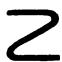
\includegraphics[keepaspectratio]{images/part001_149bf36b.jpg}}

Thus, if E is locally convex and metrizable, and if its topology cannot be defined by a single norm, then there exists no distance on E defining its topology and such that the bounded subsets for \(d\) (GT, IX, § 2, No.~2) are the bounded subsets of E. More precisely, for every distance \(d\) on E, which is translation invariant and which defines the topology of E, the bounded subsets of E are bounded for \(d\) (III, p.~38, exerc. 3), but the converse is false.

\begin{enumerate}
\def\labelenumi{\arabic{enumi})}
\setcounter{enumi}{1}
\item
  Let M be a vector subspace of E endowed with the induced topology. In order that a subset of M be bounded in M, it is necessary and sufficient that it be bounded in E.
\item
  Let N be the intersection of all neighbourhoods of 0 in E, so that \(\tilde{E} = E/N\) is the Hausdorff vector space associated with E. Then N is bounded; if \(\pi: E \to \tilde{E}\) is the canonical homomorphism then a subset B of E is bounded if and only if \(\pi(B)\) is bounded.
\item
  Let E be a Hausdorff locally convex space; then for every \(x \neq 0\) in E, there exists a continuous semi-norm p such that \(p(x) \neq 0\) ; this semi-norm is not bounded on the real half-line \(R_{+}.x\) generated by x. Hence no non-null subspace of E is bounded. In particular, a bounded subset does not contain any line.
\end{enumerate}

DEFINITION 4. --- Let E be a locally convex space. A bornology B on E is said to be adapted to E, if it is convex, is composed of bounded subsets of E and if the closure of every set of B belongs to B.

PROPOSITION 1. --- Let E be a locally convex space. The set of bounded subsets of E is an adapted bornology.

We need to establish the following properties :

\begin{enumerate}
\def\labelenumi{\alph{enumi})}
\item
  If \(\mathbf{B}\) is a bounded subset of \(\mathbf{E}\) , every subset of \(\mathbf{B}\) is bounded.
\item
  The union of two bounded subsets is bounded.
\item
  Every set that is homothetic to a bounded set is bounded.
\item
  The closed convex balanced envelope (II, p.~13) of a bounded subset is bounded.
\end{enumerate}

If p is a continuous semi-norm on E, the balls of p are convex, balanced, closed and the set homothetic to a ball is a ball. Hence, if p is bounded on two subsets X and Y of E, it is also bounded on the closed convex balanced envelope of \(X \cup Y\) , and on the sets homothetic to these. This establishes properties b), c) and d), and a) is obvious.

DEFINITION 5. --- Let E be a locally convex space. The set of all bounded subsets of E is called the canonical bornology of E.

If B is a set of bounded subsets of E, then there exists a smallest bornology \(\tilde{B}\) adapted to E and containing B. The sets of \(\tilde{B}\) are those that are contained in a set homothetic to the closed convex balanced envelope of a finite union of sets of B.

Every adapted bornology is contained in the canonical bornology.

PROPOSITION 2. --- In a locally convex space E, every precompact set is bounded. Let A be a precompact subset of E, and V be a convex balanced neighbourhood of 0. There exists a finite sequence \((a_{i})_{1\leqslant i\leqslant n}\) of points of A such that

\[
\mathrm{A} \subset \bigcup_ {1 \leqslant i \leqslant n} (a _ {i} + \mathrm{V}).
\]

Since \(B = \{a_{1}, ..., a_{n}\}\) is bounded, there exists a scalar \(\lambda\) such that \(0 < \lambda < 1\) and \(\lambda B \subset V\) ; we have \(\lambda A \subset \lambda B + \lambda V \subset V + V\) , from which the proposition follows.

COROLLARY. --- In a locally convex space, the set of points of a Cauchy sequence is bounded.

In fact, this set is precompact (GT, II, § 4, No.~2).

Remark 5. --- In general the bounded subsets of a locally convex space E are not all precompact (for example, if E is an infinite dimensional normed space, its unit ball is not compact (I, p.~15, th. 3)). However, this is so if E is a weak space (II, p.~42) : for the Hausdorff topological vector space associated with E is then isomorphic to a subspace of a product \(K^{I}\) whose bounded subsets are precompact (cf.~III, p.~4, cor. 2).

For other examples, see IV, p.~18.

PROPOSITION 3. --- Let A be a subset of a locally convex space E. Suppose that A is bounded; then for every sequence \((x_{n})\) of points of A and for every sequence \((\lambda_{n})\) of scalars tending to 0, the sequence \((\lambda_{n}x_{n})\) tends to 0. Conversely, if there exists a sequence \((\lambda_{n})\) of non-zero scalars such that for every sequence \((x_{n})\) of points of A, the sequence \((\lambda_{n}x_{n})\) is bounded, then A is bounded.

Suppose that A is bounded. If \((\lambda_{n})\) is a sequence of scalars tending to 0, and V is a neighbourhood of 0, we have \(\lambda_{n}A \subset V\) whenever n is large enough, and the first assertion follows.

Conversely, if A is not bounded and if \((\lambda_{n})\) is a sequence of scalars \(\neq 0\) , then there exists a continuous semi-norm p and a sequence \((x_{n})\) of points of A, such that \(p(x_{n}) \geqslant \frac{n}{|\lambda_{n}|}\) . We have then that \(p(\lambda_{n}x_{n}) \geqslant n\) , and the sequence \((\lambda_{n}x_{n})\) is not bounded.

COROLLARY. --- A subset A of E is bounded if and only if every countable subset of A is bounded.

\subsection{Image under a continuous mapping}

PROPOSITION 4. --- Let E and F be two locally convex spaces and \(f:E \rightarrow F\) a continuous mapping. Assume that \(f(0) = 0\) and that there exists a real number \(m \geqslant 0\) such that \(f(\lambda x) = \lambda^{m}f(x)\) for every \(\lambda > 0\) . Then, if A is a bounded subset of E, \(f(A)\) is bounded in F.

In fact, if V is a neighbourhood of 0 in F, then \(f^{-1}(V)\) is a neighbourhood of 0 in E. If A is bounded in E, there exists \(\lambda > 0\) such that \(A \subset \lambda f^{-1}(V)\) and this implies that \(f(A) \subset \lambda^{m}V\) .

COROLLARY 1. --- Let E and F be two locally convex spaces, and \(u:E\to F\) be a continuous linear mapping. If A is a bounded subset of E, then \(u(A)\) is bounded in F.

COROLLARY 2. --- Let \(\mathrm{E} = \prod_{i\in \mathrm{I}}\mathrm{E}_i\) be the product of a family of locally convex spaces.

Then a subset of E is bounded if and only if all its projections are bounded. More generally :

COROLLARY 3. --- Let E be a vector space, \((\mathrm{F}_{i})_{i\in\mathrm{I}}\) a family of locally convex spaces and \(f_{i}\) a linear mapping from E into \(F_{i}\) (for \(i\in I\) ). Suppose E is assigned the coarsest topology (locally convex) for which all the \(f_{i}\) are continuous (II, p.~26). Then, for a subset A of E to be bounded, it is necessary and sufficient that \(f_{i}(A)\) is bounded in \(F_{i}\) for all \(i\in I\) .

In fact, if A is bounded, so are the \(f_{i}(\mathbf{A})\) (cor. 1). Conversely, if the \(f_{i}(\mathbf{A})\) are bounded and if p is a continuous semi-norm on E, then there exists a finite subset J of I and a family \((q_{j})_{j\in \mathbb{J}}\) , where \(q_{j}\) is a continuous semi-norm on \(\mathbf{F}_j\) , such that \(p\leqslant \sup_{j\in \mathbb{J}}(q_j\circ f_j)\) consequently \(p\) is bounded on \(\mathbf{A}\) .

COROLLARY 4. --- Let \(\mathbf{E}_i\) ( \(1 \leqslant i \leqslant n\) ) and \(\mathbf{F}\) be locally convex spaces, and \(f\) be a continuous multilinear map from \(\prod_{i=1}^{n} \mathbf{E}_i\) into \(\mathbf{F}\) . If \(\mathbf{B}_i\) is a bounded subset of \(\mathbf{E}_i\) , for \(1 \leqslant i \leqslant n\) , then \(f\left(\prod_{i=1}^{n} \mathbf{B}_i\right)\) is bounded in \(\mathbf{F}\) .

COROLLARY 5. --- Let E and F be two locally convex spaces and \(u:E\to F\) be a continuous polynomial mapping. If A is a bounded subset of E, then \(u(A)\) is bounded.

\subsection{Bounded subsets in certain inductive limits}

PROPOSITION 5. --- Let \((\mathrm{E}_{i})_{i\in\mathbf{I}}\) be a family of Hausdorff locally convex spaces, and let E be the topological direct sum of this family (II, p.~29). In order that a subset B of E be bounded, it is necessary and sufficient that there exists a finite subset J of I such that \(\operatorname{pr}_{i}(\mathbf{B})\) is bounded in \(E_{i}\) for \(i\in J\) and \(\operatorname{pr}_{i}(\mathbf{B})\subset\{0\}\) for all \(i\notin J\) .

Let J be a finite subset of I. Since the topology of E induces the product topology on \(\prod_{j\in J}E_{j}\) (II, p.~30, prop. 7 and p.~31, prop. 8), it follows from III, p.~4, cor. 2 that the condition is sufficient.

Conversely, let B be a bounded subset of E. Then \(\mathrm{pr}_{i}(\mathbf{B})\) is bounded for all i (III, p.~4, cor. 1). Therefore it is enough to prove that there exists a finite subset J of I such that \(\mathrm{pr}_{i}(\mathbf{B}) \subset \{0\}\) for all \(i \notin J\) . If not, then there exists an infinite sequence \((i_{n})\) of distinct elements of I and an infinite sequence \((x_{n})\) of elements of B such that \(\mathrm{pr}_{i_{n}}(x_{n}) \neq 0\) . Since \(E_{i_{n}}\) is Hausdorff, there exists a continuous semi-norm \(p_{n}\) on \(E_{i_{n}}\) such that \(p_{n}(\mathrm{pr}_{i_{n}}(x_{n})) \geqslant n\) . Hence \(p = \sum_{n \geqslant 1} p_{n} \circ \mathrm{pr}_{i_{n}}\) is a continuous semi-norm on E and p is not bounded on B, which is a contradiction.

PROPOSITION 6. --- Let E be a locally convex space which is the strict inductive limit of an increasing sequence \((E_{n})\) of closed vector subspaces of E (II, p.~33). A subset B of E is bounded if and only if it is contained in one of the subspaces \(E_{n}\) , and is bounded in this subspace.

The condition is sufficient, since the topology induced on \(E_{n}\) by that of E is precisely the given topology of \(E_{n}\) (II, p.~32, prop. 9). To see that the condition is necessary, it is enough (III, p.~4, prop. 3) to prove that if a sequence \((x_{m})\) of points of E is not contained in any of the subspaces \(E_{n}\) , then it cannot tend to 0. By extracting a subsequence of the sequence \((x_{m})\) , we can assume that there exists a strictly increasing sequence \((n_{k})\) of integers such that, for every index k, we have \(x_{k} \notin E_{n_{k}}\) and \(x_{k} \in E_{n_{k+1}}\) . Then there exists (II, p.~33, lemma 2) an increasing sequence \((V_{k})\) of convex sets such that \(V_{k}\) is a neighbourhood of 0 in \(E_{n_{k}}\) , \(V_{k+1} \cap E_{n_{k}} = V_{k}\) and such that \(x_{k} \notin V_{k+1}\) for every index k. The union V of the \(V_{k}\) is then a neighbourhood of 0 in E, and we have \(x_{k} \notin V\) for all k. This proves that the sequence \((x_{k})\) does not tend to 0.

The conclusion of prop. 6 is not necessarily true for a space \(\mathbf{E}\) which is the inductive limit of a non-denumerable directed set of closed subspaces of \(\mathrm{E}\) (cf.~III, p.~38, exerc. 7).

PROPOSITION 7. --- Let \((\mathrm{E}_{n})_{n\geq0}\) be a sequence of Hausdorff locally convex spaces, and for every n, let \(u_{n}:E_{n}\to E_{n+1}\) be an injective linear mapping which is compact (i.e.~such that there exists a neighbourhood of 0 in \(E_{n}\) whose image under \(u_{n}\) is relatively compact; this implies that \(u_{n}\) is continuous). Let E be the inductive limit of the system \((\mathrm{E}_{n},u_{n})\) (II, p.~29), and let \(v_{n}\) be the canonical mapping from \(E_{n}\) into E. Then the locally convex space E is Hausdorff. Moreover, for every subset A of E, the following conditions are equivalent :

\begin{enumerate}
\def\labelenumi{(\roman{enumi})}
\item
  A is bounded;
\item
  there exists an integer \(n\) such that \(\mathbf{A}\) is the image under \(v_{n}\) of a bounded subset of \(\mathrm{E}_n\) ;
\item
  A is relatively compact.
\end{enumerate}

We identify \(\mathbf{E}_n\) with a vector subspace of \(\mathbf{E}\) (endowed with a topology finer than the induced topology).

Lemma 1. --- Under the hypothesis of prop. 7, the topology of E is the finest topology for which all the mappings \(v_{n} : \mathrm{E}_{n} \to \mathrm{E}\) are continuous.

We need to prove that, if U is a subset of E such that \(U \cap E_{n}\) is open in \(E_{n}\) for every n, then U is open in E; in other words, we must prove that, for every \(x \in U\) , there exists a convex balanced set V such that \(x + V \subset U\) and that \(V \cap E_{n}\) is a neighbourhood of 0 in \(E_{n}\) for every large enough n (II, p.~27, prop. 5). For every n, let \(W_{n}\) be a convex balanced neighbourhood of 0 in \(E_{n}\) such that the closure \(H_{n}\) of \(W_{n}\) in \(E_{n+1}\) is compact. Let \(x \in U\) and let \(n_{0}\) be an integer such that \(x \in E_{n_{0}}\) . We shall construct, by induction, a sequence \((\varepsilon_{n})_{n \geqslant 0}\) of scalars \textgreater0 such that \(x + \sum_{n_{0} \leqslant i \leqslant n} \varepsilon_{i}H_{i}\) is contained in U for \(n \geqslant n_{0}\) . Suppose that the \(\varepsilon_{i}\) for i \textless{} n have been constructed. If \(n = n_{0}\) , set \(V_{n-1} = \{0\}\) ; if not, set

\[
\mathrm{V} _ {n - 1} = \sum_ {n _ {0} \leqslant i \leqslant n - 1} \varepsilon_ {i} \mathrm{H} _ {i}.
\]

Then \(V_{n-1}\) is compact in \(E_{n}\) , and a fortiori in \(E_{n+1}\) . Since \(U \cap E_{n+1}\) is open in \(E_{n+1}\) , there exists a scalar \(\varepsilon_{n} > 0\) such that \(x + V_{n} = x + V_{n-1} + \varepsilon_{n}H_{n}\) is contained in U (GT, II, §4, No.~3, cor.). Let \(V = \bigcup_{n \geqslant n_{0}} V_{n}\) . Then V is convex and balanced; for \(n \geqslant n_{0}\) , we have \(V \cap E_{n} \supset \varepsilon_{n}H_{n} \cap E_{n} \supset \varepsilon_{n}W_{n}\) , hence \(V \cap E_{n}\) is a neighbourhood of 0 in \(E_{n}\) . This completes the proof of the lemma.

The set \(\mathrm{U} = \mathrm{E} - \{0\}\) is such that the set \(\mathrm{U} \cap \mathrm{E}_n = \mathrm{E}_n - \{0\}\) is open in \(\mathrm{E}_n\) for every \(n\) , hence \(\mathrm{U}\) is open in \(\mathrm{E}\) , which proves that \(\mathrm{E}\) is Hausdorff (GT, III, § 1, No.~3, prop. 2). It is clear that property (ii) implies (iii) and that (iii) implies (i). Finally we show that (i) implies (ii). For this it is enough to show that if a subset \(\mathrm{A}\) of \(\mathrm{E}\) is not absorbed by any of the sets \(\sum_{0 \leqslant i \leqslant n} \mathrm{H}_i\) , then \(\mathrm{A}\) is not bounded. But then there exists a sequence \((x_n)_{n \geqslant 1}\) of points of \(\mathrm{A}\) such that, for every \(n\) , we have \(x_n \notin n^2 \sum_{0 \leqslant i \leqslant n} \mathrm{H}_i\) .

Then the set of the \(x_{n}/n\) is closed by virtue of lemma 1, since its intersection with \(E_{m}\) is discrete for every integer m. The complement of the set of the \(x_{n}/n\) is then an open neighbourhood of 0 which does not absorb the sequence \((x_{n})\) , hence A is not bounded.

Remarks. --- 1) With the above notations, let \(F_{n}\) be the vector space generated by \(H_{n}\) , with a norm equal to the gauge of \(H_{n}\) . We shall see (III, p.~8, cor.) that \(F_{n}\) is a Banach space. The injection from \(F_{n}\) into \(E_{n+1}\) is compact, hence a fortiori also the injection \(w_{n}\) from \(F_{n}\) into \(F_{n+1}\) . Further, E is the inductive limit of the inductive system ( \(F_{n}, w_{n}\) ) of Banach spaces. For, a convex balanced neighbourhood V of 0 in E is such that \(V \cap E_{n}\) absorbs \(H_{n-1}\) for all \(n \geqslant 1\) , and conversely, if a convex balanced set W in E is such that \(W \cap E_{n}\) absorbs \(H_{n-1}\) , then \(W \cap E_{n-1}\) contains a set homothetic to \(W_{n-1}\) for all \(n \geqslant 1\) , and hence W is a neighbourhood of 0 in E.

\begin{enumerate}
\def\labelenumi{\arabic{enumi})}
\setcounter{enumi}{1}
\tightlist
\item
  Let F be a locally convex space, k an integer \(\geqslant0\) and \(f:E^{k}\rightarrow F\) a multilinear mapping. For f to be continuous, it is necessary and sufficient that the restriction of f to \(E_{n}^{k}\) is continuous for every n.~We verify immediately that \(E^{k}\) has the final locally convex topology for the family of linear mappings \(v_{n}\times\cdots\times v_{n}:E_{n}\times\cdots\times E_{n}\to E\times\cdots\times E\) (II, p.~28, cor. 2 and p.~30, prop. 7) and that \(u_{n}\times\cdots\times u_{n}\) is a compact injective linear mapping from \((\mathrm{E}_{n})^{k}\) into \((\mathrm{E}_{n+1})^{k}\) . It is now enough to apply lemma 1.
\end{enumerate}
